

\chapter{Kiến trúc đa nền tảng}
\begin{flushleft}
    \hspace*{0.8cm}Với sự phát triển mạnh mẽ của thị trường di động và nhu cầu ngày càng cao về ứng dụng chạy trên nhiều hệ điều hành, kiến trúc đa nền tảng đã trở thành một giải pháp quan trọng giúp giảm chi phí và thời gian phát triển. Các framework như React Native và Flutter nổi bật trong việc cho phép tái sử dụng mã nguồn lên tới 50--80\% giữa các nền tảng iOS và Android, từ đó tối ưu quy trình phát triển và bảo trì ứng dụng. Tuy nhiên, mỗi framework lại có những đặc điểm và ưu nhược điểm riêng. React Native sử dụng JavaScript và có hệ sinh thái mạnh mẽ, dễ tích hợp vào các hệ thống web, trong khi Flutter với ngôn ngữ Dart và engine Skia mang đến hiệu suất cao và khả năng tùy biến giao diện vượt trội. Dù vậy, sự lựa chọn giữa hai framework này không chỉ phụ thuộc vào yếu tố kỹ thuật mà còn phải cân nhắc về các yêu cầu cụ thể của dự án, như hiệu suất, khả năng mở rộng và mức độ phức tạp của giao diện người dùng. Các nhà phát triển cần đánh giá kỹ lưỡng các yếu tố này để chọn ra giải pháp phù hợp nhất cho từng dự án, tối ưu hóa chi phí và thời gian phát triển.
\end{flushleft}
\label{chap:Chap4}

\section{Giới thiệu}
  
    \hspace*{0.8cm}Trong bối cảnh số lượng người dùng thiết bị di động không ngừng tăng, nhu cầu phát triển ứng dụng hoạt động mượt mà trên cả iOS và Android ngày càng trở nên cấp thiết. Kiến trúc đa nền tảng (cross-platform) đã nổi lên như một giải pháp giúp doanh nghiệp tối ưu chi phí, rút ngắn thời gian phát hành và đơn giản hóa quy trình bảo trì so với phương pháp native truyền thống. Các framework như React Native và Flutter cho phép tái sử dụng 50--80\% mã nguồn, đồng thời cung cấp công cụ phát triển hiện đại như hot reload và bộ widget tùy biến cao. Nghiên cứu này tập trung phân tích ưu nhược điểm của hai framework trên qua các khía cạnh: hiệu năng (FPS, RAM), chi phí, thời gian triển khai và khả năng ứng dụng vào các loại dự án khác nhau, từ đó đề xuất tiêu chí lựa chọn phù hợp cho từng trường hợp sử dụng cụ thể.  
\vspace{0.5em}

\subsection{Bối cảnh nghiên cứu}
\renewcommand{\labelitemi}{--}    

    \hspace*{0.8cm}Sự phát triển nhanh chóng của thị trường di động trong những năm gần đây đã làm thay đổi đáng kể cách thức xây dựng ứng dụng. Theo báo cáo của Statista (2023)~\cite{statista2023}, số lượng người dùng smartphone toàn cầu đạt 6.92 tỷ vào năm 2023 và dự kiến sẽ tăng lên 7.5 tỷ vào năm 2025. Trước thực tế này, các nhà phát triển đứng trước bài toán lớn: làm thế nào để tạo ra ứng dụng chạy trơn tru trên cả iOS và Android mà không cần xây dựng hai hệ thống riêng biệt?
\vspace{0.5em}


    \hspace*{0.8cm}Phát triển ứng dụng native cho từng nền tảng từng là giải pháp phổ biến, nhưng nó kéo theo chi phí cao, thời gian dài và yêu cầu nguồn nhân lực lớn. Ví dụ, một công ty startup có thể mất tới 18 tháng và khoảng 500.000 USD để xây dựng song song hai ứng dụng native cho iOS và Android.
\vspace{0.5em}


    \hspace*{0.8cm}Chỉ riêng chi phí nhân sự đã là gánh nặng: theo Business of Apps~\cite{businessofapps2025}, mức lương trung bình hàng năm của lập trình viên ứng dụng di động tại Mỹ dao động từ 80.000 đến 150.000 USD, tùy thuộc vào công nghệ và kinh nghiệm. Ví dụ, lập trình viên Flutter có thể nhận khoảng 7.800 USD/tháng, trong khi React Native là khoảng 8.000 USD/tháng. Với hai lập trình viên làm việc trong 18 tháng, tổng chi phí nhân sự có thể lên đến 280.000--350.000 USD, chưa kể đến chi phí thiết kế, kiểm thử và quản lý dự án.
\vspace{0.5em}


    \hspace*{0.8cm}Để giải quyết những hạn chế này, các công nghệ phát triển ứng dụng đa nền tảng (cross-platform) bắt đầu nổi lên như một giải pháp tiềm năng. Kể từ khi Facebook giới thiệu React Native vào năm 2015, lập trình viên đã có thể sử dụng JavaScript để viết giao diện và logic nghiệp vụ, từ đó giảm thiểu đáng kể lượng mã cần viết riêng cho từng hệ điều hành. Tiếp đó, năm 2017, Google ra mắt Flutter, framework sử dụng ngôn ngữ Dart và engine Skia, cho phép render UI trực tiếp mà không phụ thuộc vào widget native.
\vspace{0.5em}


    \hspace*{0.8cm}Nhờ khả năng tái sử dụng mã nguồn lên tới 50--80\% giữa hai nền tảng, giải pháp cross-platform giúp các startup cắt giảm 30--40\% chi phí phát triển so với native thuần túy. Báo cáo của Cleveroad~\cite{cleveroad} cũng ghi nhận rằng, chi phí phát triển ứng dụng đa nền tảng thường dao động từ 60.000--200.000 USD, thấp hơn đáng kể so với mức 70.000--250.000 USD nếu phát triển từng ứng dụng riêng biệt. Không chỉ tiết kiệm ngân sách, thời gian đưa sản phẩm ra thị trường cũng được rút ngắn nhờ sử dụng chung codebase và quy trình kiểm thử tập trung. Ví dụ, một ứng dụng phức tạp thường mất 7--16 tuần để phát triển native độc lập, nhưng chỉ cần 11--20 tuần với React Native hoặc Flutter, nhờ tính năng hot reload và workflow thống nhất.
\vspace{0.5em}


    \hspace*{0.8cm}Tổng thể, thay vì mất 18 tháng và 500.000 USD, các công ty hiện nay chỉ cần 12--14 tháng và khoảng 200.000--250.000 USD để hoàn thiện sản phẩm cho cả hai nền tảng, thể hiện rõ ưu thế của các framework cross-platform trong việc tối ưu chi phí và thời gian phát triển.
\vspace{0.5em}


    \hspace*{0.8cm}Theo khảo sát của Stack Overflow (2023)~\cite{stackoverflow2023}, Flutter hiện được 42\% nhà phát triển ưu tiên lựa chọn, trong khi React Native chiếm 38\%. Sự cạnh tranh giữa hai framework này không chỉ phản ánh xu hướng ``Write Once, Run Anywhere'' mà còn đặt ra câu hỏi mới về hiệu năng, khả năng mở rộng và tùy biến trong các ứng dụng hiện đại.
\vspace{0.5em}

\subsection{Mục tiêu nghiên cứu}
\renewcommand{\labelitemi}{--}    

    \hspace*{0.8cm}Bài nghiên cứu này hướng đến ba mục tiêu chính:
    \setlength{\leftmargini}{1.0cm}
    \begin{itemize}
        \item Mục tiêu thứ nhất là phân tích ưu điểm và hạn chế của kiến trúc đa nền tảng so với phát triển native, nhằm đánh giá khả năng tiết kiệm chi phí, rút ngắn thời gian phát triển, đồng thời nhận diện các thách thức liên quan đến hiệu năng và trải nghiệm người dùng.
        \item Mục tiêu thứ hai là đo lường và phân tích các rào cản về mặt kỹ thuật của ứng dụng đa nền tảng, thông qua các chỉ số như tốc độ khung hình (FPS), mức tiêu thụ RAM, và thời gian phản hồi. Từ đó, so sánh các giá trị này với ứng dụng native để xác định mức độ chênh lệch rõ ràng.
        \item Mục tiêu thứ ba là đề xuất tiêu chí lựa chọn framework phù hợp với từng loại dự án, dựa trên ngân sách, thời gian triển khai và đặc thù ứng dụng. Ví dụ, Flutter có thể phù hợp với ứng dụng thiên về đồ họa như game, trong khi React Native có thể là lựa chọn tối ưu cho ứng dụng doanh nghiệp.
    \end{itemize}
\vspace{0.5em}

\subsection{Phạm vi và đối tượng}
\renewcommand{\labelitemi}{--}    

    \hspace*{0.8cm}Phạm vi nghiên cứu tập trung vào hai framework hàng đầu trong phát triển ứng dụng đa nền tảng hiện nay, bao gồm:
    \setlength{\leftmargini}{1.0cm}
    \begin{itemize}
        \item \textbf{React Native}, do Facebook phát triển, dựa trên ngôn ngữ JavaScript. Framework này nổi bật nhờ hệ sinh thái mở rộng (npm, Expo) và khả năng tích hợp dễ dàng vào các hệ thống web sẵn có.
        \item \textbf{Flutter}, do Google phát triển, sử dụng ngôn ngữ Dart. Framework này được đánh giá cao nhờ hiệu năng vượt trội và khả năng tùy biến giao diện người dùng thông qua engine Skia.
    \end{itemize}
\vspace{0.5em}


    \hspace*{0.8cm}Lý do lựa chọn hai framework này đến từ vị thế dẫn đầu thị trường của chúng:
    \setlength{\leftmargini}{1.0cm}
    \begin{itemize}
        \item Theo báo cáo của SlashData (2023)~\cite{slashdata2023}, React Native và Flutter chiếm đến 80\% thị phần framework đa nền tảng.
        \item Cả hai đều sở hữu cộng đồng lập trình viên lớn, tài liệu kỹ thuật phong phú, và đã được triển khai rộng rãi trong các dự án thực tế.
    \end{itemize}
\vspace{0.5em}


    \hspace*{0.8cm}Nguồn dữ liệu trong nghiên cứu được tổng hợp từ các công trình thực nghiệm uy tín:
    \setlength{\leftmargini}{1.0cm}
    \begin{itemize}
        \item \textbf{Nghiên cứu của Wenhao (2018)}~\cite{wenhao2018} tập trung vào đo hiệu năng FPS khi cuộn màn hình trên 10 ứng dụng mẫu. Kết quả cho thấy: \textit{Flutter đạt 60 FPS}, trong khi \textit{React Native đạt 45–50 FPS}.
        \item \textbf{Báo cáo của Biorn-Hansen (2021)}~\cite{biornhansen2021} đánh giá mức tiêu thụ RAM và CPU trên 15 ứng dụng thương mại. Kết quả cho thấy: \textit{Ứng dụng native sử dụng trung bình 150MB RAM}, so với \textit{200MB của Flutter} và \textit{180MB của React Native}.
    \end{itemize}
\vspace{0.5em}


    \hspace*{0.8cm}Giới hạn của nghiên cứu cũng được xác định rõ ràng:
    \setlength{\leftmargini}{1.0cm}
    \begin{itemize}
        \item Các framework ít phổ biến như Xamarin hay Ionic không nằm trong phạm vi phân tích.
        \item Các số liệu hiệu năng được thực hiện trong môi trường thử nghiệm, do đó có thể khác biệt so với khi triển khai thực tế.
    \end{itemize}
\vspace{0.5em}


    \hspace*{0.8cm}Phần giới thiệu khép lại bằng định hướng ứng dụng của nghiên cứu:
    \setlength{\leftmargini}{1.0cm}
    \begin{itemize}
        \item Việc lựa chọn kiến trúc đa nền tảng không chỉ dựa trên công nghệ, mà còn phụ thuộc vào mục tiêu kinh doanh và nguồn lực của doanh nghiệp. Nghiên cứu này hướng đến cung cấp cái nhìn toàn diện về React Native và Flutter, giúp nhà phát triển đưa ra quyết định dựa trên dữ liệu định lượng và phân tích chuyên sâu.
    \end{itemize}
\vspace{0.5em}


\section{Cơ Sở Lý Thuyết }

  Trong quá trình phát triển phần mềm hiện đại, kiến trúc hệ thống đóng vai trò then chốt trong việc đảm bảo hiệu quả và khả năng mở rộng của ứng dụng. Đặc biệt đối với các ứng dụng di động, việc lựa chọn kiến trúc phù hợp có thể ảnh hưởng trực tiếp đến chi phí, thời gian phát triển và trải nghiệm người dùng cuối. Trong phần này, chúng tôi trình bày các khái niệm nền tảng liên quan đến kiến trúc đa nền tảng như một hướng tiếp cận thay thế cho phát triển native truyền thống.
% 2.1
\subsection{Khái niệm kiến trúc đa nền tảng}
\renewcommand{\labelitemi}{--}

\subsubsection{Định nghĩa}

    Kiến trúc đa nền tảng (cross-platform architecture) là một phương pháp phát triển ứng dụng dựa trên một bộ mã nguồn chung, giúp triển khai đồng thời trên nhiều hệ điều hành như iOS, Android, cũng như các nền tảng khác như web hoặc desktop. Thay vì xây dựng từng phiên bản riêng biệt cho từng hệ điều hành, lập trình viên sử dụng các framework hoặc công cụ trung gian để biên dịch mã nguồn và tối ưu hóa cho từng môi trường cụ thể.
\vspace{0.5em}


    Các framework tiêu biểu cho kiến trúc đa nền tảng bao gồm:
    \setlength{\leftmargini}{1.5cm}
    \begin{itemize}
        \item \textbf{React Native}: Sử dụng JavaScript và biên dịch mã qua "bridge" thành mã máy tương ứng (Objective-C/Swift cho iOS, Java/Kotlin cho Android).
        \item \textbf{Flutter}: Dựa trên ngôn ngữ Dart và sử dụng Skia Engine để render giao diện trực tiếp, độc lập với hệ điều hành.
    \end{itemize}

\subsubsection{Nguyên tắc "Write Once, Run Anywhere"-(WORA)}

    Nguyên tắc WORA, được Sun Microsystems giới thiệu từ thập niên 1990, nhấn mạnh vào khả năng tái sử dụng mã nguồn tối đa và giảm chi phí phát triển. Nguyên tắc này dựa trên hai yếu tố cốt lõi:
    \setlength{\leftmargini}{1.5cm}
    \begin{itemize}
        \item \textbf{Tính độc lập nền tảng}: Mã nguồn không bị phụ thuộc vào hệ điều hành hoặc phần cứng cụ thể.
        \item \textbf{Tính nhất quán}: Logic nghiệp vụ và giao diện hoạt động đồng bộ trên mọi thiết bị.
    \end{itemize}
\vspace{0.5em}


    Một số ứng dụng thực tế đã áp dụng hiệu quả nguyên tắc này:
    \setlength{\leftmargini}{1.5cm}
    \begin{itemize}
        \item \textbf{Microsoft Teams}: Dùng React Native để triển khai trên iOS, Android và Windows với hơn 90\% mã nguồn dùng chung.
        \item \textbf{Google Pay}: Xây dựng trên Flutter, hỗ trợ cả mobile và web từ một codebase duy nhất.
    \end{itemize}

\subsubsection{Lợi ích của kiến trúc đa nền tảng}

    So với phát triển native, kiến trúc đa nền tảng mang lại nhiều lợi ích về mặt chi phí, thời gian và khả năng bảo trì:
    \setlength{\leftmargini}{1.5cm}
    \begin{itemize}
        \item \textbf{Tiết kiệm thời gian và chi phí}: Theo Intelivita (2024) ~\cite{infoq2022}, thời gian phát triển có thể giảm 30-40\%, đồng thời chỉ cần một đội ngũ phát triển thay vì nhiều nhóm chuyên biệt.
        \item \textbf{Bảo trì dễ dàng}: Việc cập nhật tính năng hoặc sửa lỗi được thực hiện một lần và áp dụng đồng thời cho mọi nền tảng.
        \item \textbf{Tích hợp CI/CD}: Quy trình phát hành được tự động hóa, giảm rủi ro và nâng cao tốc độ triển khai.
    \end{itemize}

\subsubsection{Thách thức và hạn chế}

    Mặc dù mang lại nhiều lợi thế, kiến trúc đa nền tảng vẫn tồn tại những điểm hạn chế nhất định:
    \setlength{\leftmargini}{1.5cm}
    \begin{itemize}
        \item \textbf{Hiệu năng thấp hơn native}: Theo Intelivita (2024)~\cite{infoq2022}, ứng dụng đa nền tảng có thể chậm hơn khi xử lý đồ họa nặng như animation hoặc game 3D.
        \item \textbf{Ví dụ}: Pokémon GO từng thử nghiệm với Unity (cross-platform) nhưng phải chuyển sang native do hiện tượng lag khi render bản đồ 3D.
        \item \textbf{Khó tùy chỉnh giao diện}: Các framework đa nền tảng sử dụng UI tổng quát, khó đáp ứng đặc trưng thiết kế như Material Design (Android) hay Cupertino (iOS).
        \item \textbf{Ví dụ}: Spotify (React Native) phải viết lại nhiều thành phần UI bằng mã native để đảm bảo trải nghiệm người dùng.
        \item \textbf{Phụ thuộc vào cộng đồng và công cụ}: Nhiều plugin do cộng đồng phát triển có thể thiếu ổn định hoặc ngừng duy trì.
        \item \textbf{Ví dụ}: React Native Maps từng gặp lỗi nghiêm trọng trên iOS 14, dẫn đến crash hàng loạt.
    \end{itemize}

\subsubsection{Công cụ phát triển}

  Phát triển ứng dụng đa nền tảng đòi hỏi lập trình viên sử dụng các công cụ chuyên biệt nhằm tối ưu quy trình xây dựng, kiểm thử và triển khai. Những công cụ này bao gồm IDE (môi trường phát triển tích hợp), bộ giả lập thiết bị, công cụ kiểm thử và hệ thống quản lý mã nguồn.

  \begin{figure}[H]
    \centering
    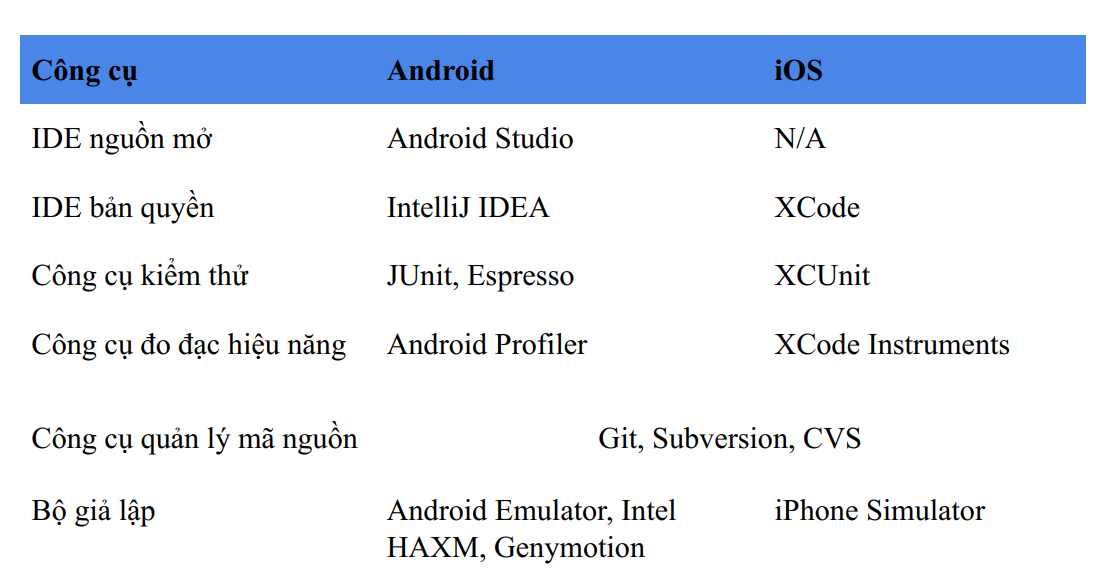
\includegraphics[width=0.95\textwidth]{images/cong-cu-android-ios.png}
    \caption{So sánh công cụ phát triển giữa Android và iOS \cite{ddiandroidios}}
    \label{fig:android_ios_tools}
  \end{figure}

  Hình~\ref{fig:android_ios_tools} thể hiện sự khác biệt giữa các công cụ được sử dụng trong hệ sinh thái Android và iOS. Việc lựa chọn công cụ phù hợp phụ thuộc vào hệ điều hành mục tiêu, ngôn ngữ lập trình và kinh nghiệm của lập trình viên.


% 2.2
\subsection{Các yếu tố quyết định khi lựa chọn đa nền tảng}
\renewcommand{\labelitemi}{--}    


  \subsubsection{Phân tích nhóm người dùng mục tiêu}
    
      Thị phần hệ điều hành đóng vai trò quan trọng trong việc xác định nền tảng ưu tiên.
      \setlength{\leftmargini}{1.5cm}
      \begin{itemize}
        \item iOS hiện chiếm 27\% thị trường toàn cầu, chủ yếu phổ biến tại Mỹ và Châu Âu.
        \item Android chiếm 73\%, đặc biệt thống trị tại Châu Á và Châu Phi (Ego-cms, 2021) ~\cite{egoMarketShare} .
      \end{itemize}
    \vspace{0.5em}

    
      Chiến lược tiếp cận người dùng cần phù hợp với đặc thù từng hệ điều hành.
      \setlength{\leftmargini}{1.5cm}
      \begin{itemize}
          \item Nếu đối tượng mục tiêu là người dùng cao cấp (iOS), nên ưu tiên framework hỗ trợ giao diện Cupertino như Flutter.
          \item Nếu nhắm tới thị trường đại chúng (Android), React Native là lựa chọn phù hợp nhờ khả năng tích hợp với Google Services.
      \end{itemize}
    \vspace{0.5em}

    
      Một ví dụ thực tế giúp minh họa rõ ràng cho lựa chọn nền tảng là Grab.
      \setlength{\leftmargini}{1.5cm}
      \begin{itemize}
          \item Grab (Flutter): Tập trung vào thị trường Đông Nam Á (đa số dùng Android) nhưng vẫn đảm bảo trải nghiệm mượt mà trên iOS.
      \end{itemize}

    \subsubsection{Mô hình "Rẻ – Nhanh – Tốt"}
    
      Nguyên tắc Iron Triangle cho rằng chỉ có thể đạt hai trong ba tiêu chí: rẻ, nhanh và tốt. Mỗi lựa chọn framework cần cân nhắc dựa trên ưu tiên này.
    \vspace{0.5em}

    \begin{figure}[H]
    \centering
    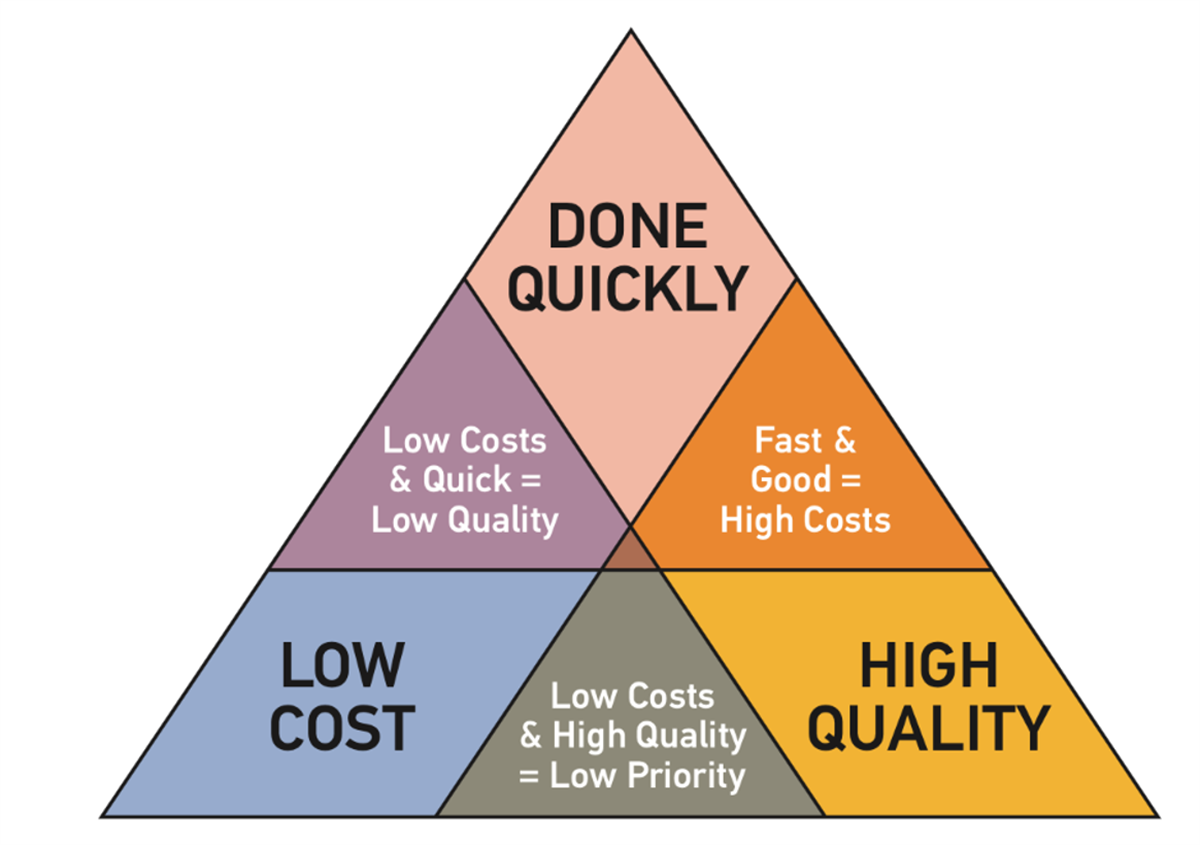
\includegraphics[width=0.45\textwidth]{images/iron_triangle.png}
    \caption{Mô hình Iron Triangle – Rẻ, Nhanh, Tốt – Chọn hai \cite{goodipidea2016}}
    \label{fig:android_ios_tools2}
  \end{figure}
    
      Tùy vào mục tiêu dự án, mỗi framework sẽ phù hợp với một chiến lược khác nhau.
      \setlength{\leftmargini}{1.5cm}
      \begin{itemize}
          \item React Native: Phù hợp cho dự án cần MVP (Minimum Viable Product) nhanh chóng, nhưng hiệu năng không cao.
          \item Flutter: Đòi hỏi đầu tư ban đầu để học Dart, nhưng mang lại hiệu năng cao và giao diện tùy biến tốt hơn.
      \end{itemize}
    

  \subsubsection{Khả năng tích hợp với hệ sinh thái hiện có}
      React Native tận dụng tốt hệ sinh thái JavaScript (Node.js, npm, Expo) và dễ tích hợp với ứng dụng web hiện tại.

      \vspace{0.5em}

      Flutter mặc dù độc lập hơn, nhưng vẫn có thể kết nối hiệu quả với Firebase hoặc Google Cloud thông qua plugin.

      \vspace{0.5em}
  
      Một ví dụ điển hình cho khả năng tích hợp là Shopify. Shopify sử dụng React Native để tích hợp ứng dụng mobile với nền tảng web sẵn có.

% 2.3
\subsection{Lịch sử phát triển của kiến trúc đa nền tảng}

\subsubsection{Thế hệ đầu tiên (2010–2015): WebView-based Frameworks}
Giai đoạn đầu tiên trong kiến trúc đa nền tảng là sự xuất hiện của các framework dựa trên WebView, điển hình là PhoneGap, Cordova, và Ionic. Các framework này hoạt động bằng cách đóng gói nội dung HTML/CSS/JavaScript trong WebView, tức bản chất ứng dụng chỉ là trình duyệt bên trong native shell.

\vspace{0.5em}

\indent Một ưu điểm lớn của các framework này là lập trình viên web có thể dễ dàng phát triển ứng dụng với chi phí phát triển và bảo trì thấp. Tuy nhiên, chúng có những hạn chế rõ ràng như hiệu năng thấp, không xử lý tốt các animation phức tạp, và giao diện thiếu tính bản địa hoá. Một ví dụ điển hình là ứng dụng Uber, ban đầu phát triển bằng Cordova nhưng phải chuyển sang native do hiện tượng lag khi hiển thị bản đồ.

\subsubsection{Thế hệ thứ hai (2015–2017): Hybrid Frameworks}

Sau WebView, thế hệ thứ hai ra đời với sự kết hợp giữa WebView và native components, gọi là Hybrid Frameworks, điển hình là Xamarin và NativeScript. Các framework này sử dụng cơ chế \textit{bridge} để kết nối JavaScript (hoặc C\#) với native APIs, cho phép sử dụng một số thành phần giao diện bản địa.

\vspace{0.5em}

\indent Hybrid frameworks mang lại hiệu năng cải thiện so với WebView và cho phép truy cập các native APIs như camera, GPS. Tuy nhiên, chúng vẫn có một số hạn chế như quá trình cấu hình phức tạp và dễ lỗi, và một số phần vẫn phải phụ thuộc vào WebView. Microsoft Outlook là ví dụ điển hình khi sử dụng Xamarin để phát triển ứng dụng đa nền tảng hiệu quả.

\subsubsection{Thế hệ hiện đại (2017–nay): Native-Reactive Frameworks}

 Từ năm 2017, kiến trúc đa nền tảng đã chuyển sang giai đoạn hiện đại với sự xuất hiện của các framework sử dụng native rendering, ví dụ như React Native và Flutter. Các framework này sử dụng cơ chế điều khiển native components thông qua bridge (React Native) hoặc tự vẽ giao diện mà không phụ thuộc vào hệ điều hành (Flutter).

\vspace{0.5em}

Nhờ cơ chế hiện đại, các framework này mang lại hiệu năng gần tương đương ứng dụng native và hỗ trợ đa nền tảng, từ mobile đến web và desktop. Một số bước đột phá quan trọng trong giai đoạn này gồm Flutter 2.0 (2020) mở rộng hỗ trợ nền tảng web và desktop, và React Native New Architecture (2022) sử dụng TurboModules và Fabric để tối ưu hiệu suất.

\vspace{0.5em}

\indent Ứng dụng Xianyu của Alibaba là ví dụ thành công khi sử dụng Flutter để phục vụ hơn 200 triệu người dùng, đạt hiệu năng tương đương ứng dụng native.
% 2.4
\subsection{Xu hướng tương lai của kiến trúc đa nền tảng}
\renewcommand{\labelitemi}{--}

\subsubsection{Tích hợp AI/ML trong phát triển}

Một trong những xu hướng quan trọng là việc tích hợp trí tuệ nhân tạo và học máy vào quy trình phát triển ứng dụng đa nền tảng. Thông qua công cụ như Google’s ML Kit, lập trình viên có thể tự động hóa các tác vụ như nhận diện hình ảnh và xử lý ngôn ngữ tự nhiên.

\vspace{0.5em}

AI không chỉ hỗ trợ tính năng thông minh, mà còn giúp tối ưu hiệu năng ứng dụng. Cụ thể, các hệ thống AI có thể phân tích mã nguồn để đề xuất cải thiện tốc độ khung hình (FPS) hoặc giảm tiêu thụ bộ nhớ RAM.

\vspace{0.5em}

Một ví dụ điển hình là Adobe XD, trong đó AI được sử dụng để tự động điều chỉnh giao diện người dùng dựa trên hành vi thực tế của người dùng.


\subsubsection{WebAssembly (Wasm) và Progressive Web Apps (PWA)}

WebAssembly đang nổi lên như một công nghệ quan trọng giúp ứng dụng chạy trên trình duyệt với hiệu năng gần tương đương ứng dụng native.  
Khả năng này giúp mở rộng phạm vi triển khai ứng dụng đa nền tảng trên môi trường web một cách hiệu quả.

\vspace{0.5em}

Cùng với đó, Progressive Web Apps (PWA) mang lại sự kết hợp giữa ứng dụng web và mobile app,  
hỗ trợ hoạt động offline và cho phép gửi thông báo đẩy đến người dùng như các ứng dụng native.

\vspace{0.5em}

Một ví dụ tiêu biểu là Starbucks, hãng đã triển khai PWA để tăng tốc độ tải trang và nâng cao trải nghiệm người dùng ngay cả khi không có kết nối mạng ổn định.


\subsubsection{Low-Code/No-Code Platforms}

Low-code và no-code platforms đang mở ra cơ hội mới cho cả những người không chuyên trong lĩnh vực lập trình. Với các nền tảng kéo–thả trực quan, người dùng có thể xây dựng ứng dụng đa nền tảng mà không cần viết bất kỳ dòng code nào.

\vspace{0.5em}

Lợi ích lớn nhất của mô hình này là rút ngắn thời gian phát triển và giảm thiểu chi phí đào tạo kỹ thuật, đặc biệt phù hợp với doanh nghiệp nhỏ hoặc bộ phận nội bộ cần triển khai nhanh giải pháp công nghệ.

\vspace{0.5em}

Chẳng hạn, Microsoft Power Apps đã giúp nhiều doanh nghiệp tạo ra ứng dụng quản lý nội bộ chỉ trong vài giờ làm việc.


% 2.5
\subsection{Case Study Chi Tiết}
\renewcommand{\labelitemi}{--}

\subsubsection{Airbnb và bài học từ React Native}

Airbnb đã từng áp dụng React Native với kỳ vọng tận dụng khả năng chia sẻ code giữa các nền tảng.  
Tuy nhiên, trong quá trình phát triển, họ gặp phải một số thách thức lớn. Cụ thể, nhóm phát triển gặp khó khăn trong việc tùy chỉnh giao diện người dùng phức tạp cho từng nền tảng, đặc biệt là khi phải đảm bảo trải nghiệm nhất quán và mượt mà. Ngoài ra, hiệu năng ứng dụng không đủ đáp ứng yêu cầu khi tích hợp tính năng đặt phòng theo thời gian thực, gây ảnh hưởng đến trải nghiệm người dùng cuối.

\vspace{0.5em}

Để giải quyết vấn đề này, Airbnb quyết định chuyển sang phát triển native cho các module quan trọng,  
đồng thời giữ lại React Native cho phần quản trị nội bộ nhằm tiết kiệm chi phí. Kết quả của chiến lược này là hiệu năng hệ thống được cải thiện 30\%,  
nhưng chi phí bảo trì cũng tăng lên khoảng 40\% do cần duy trì song song hai mã nguồn.

\subsubsection{Google Pay: Thành công với Flutter}

Google Pay là một trong những ví dụ điển hình cho việc ứng dụng thành công Flutter vào phát triển đa nền tảng. Chiến lược của nhóm phát triển là sử dụng một codebase duy nhất cho cả iOS, Android và web.

\vspace{0.5em}

Nhờ khả năng đồng bộ cao của Flutter, thời gian phát triển đã giảm tới 50\%, giúp nhóm ra mắt sản phẩm nhanh hơn mà vẫn đảm bảo chất lượng. Bên cạnh đó, hiệu năng ứng dụng cũng được đảm bảo, với tốc độ khung hình (FPS) ổn định ở mức 60 trên mọi thiết bị, tạo nên trải nghiệm người dùng mượt mà và đáng tin cậy.

\vspace{0.5em}

Tuy nhiên, nhóm cũng đối mặt với thách thức trong việc đào tạo đội ngũ kỹ thuật,  
đặc biệt là làm quen với ngôn ngữ Dart và cơ chế vẽ giao diện qua Skia Engine.

% 2.6
\subsection{So Sánh Chi Tiết React Native vs. Flutter}
\renewcommand{\labelitemi}{--}    

    Biểu đồ dưới đây so sánh mức độ quan tâm giữa hai framework di động phổ biến: \textbf{Flutter (xanh)} và \textbf{React Native (đỏ)} trong 12 tháng qua tại Hoa Kỳ, dựa trên dữ liệu tìm kiếm từ Google Trends.

    \begin{figure}[H]
        \centering
        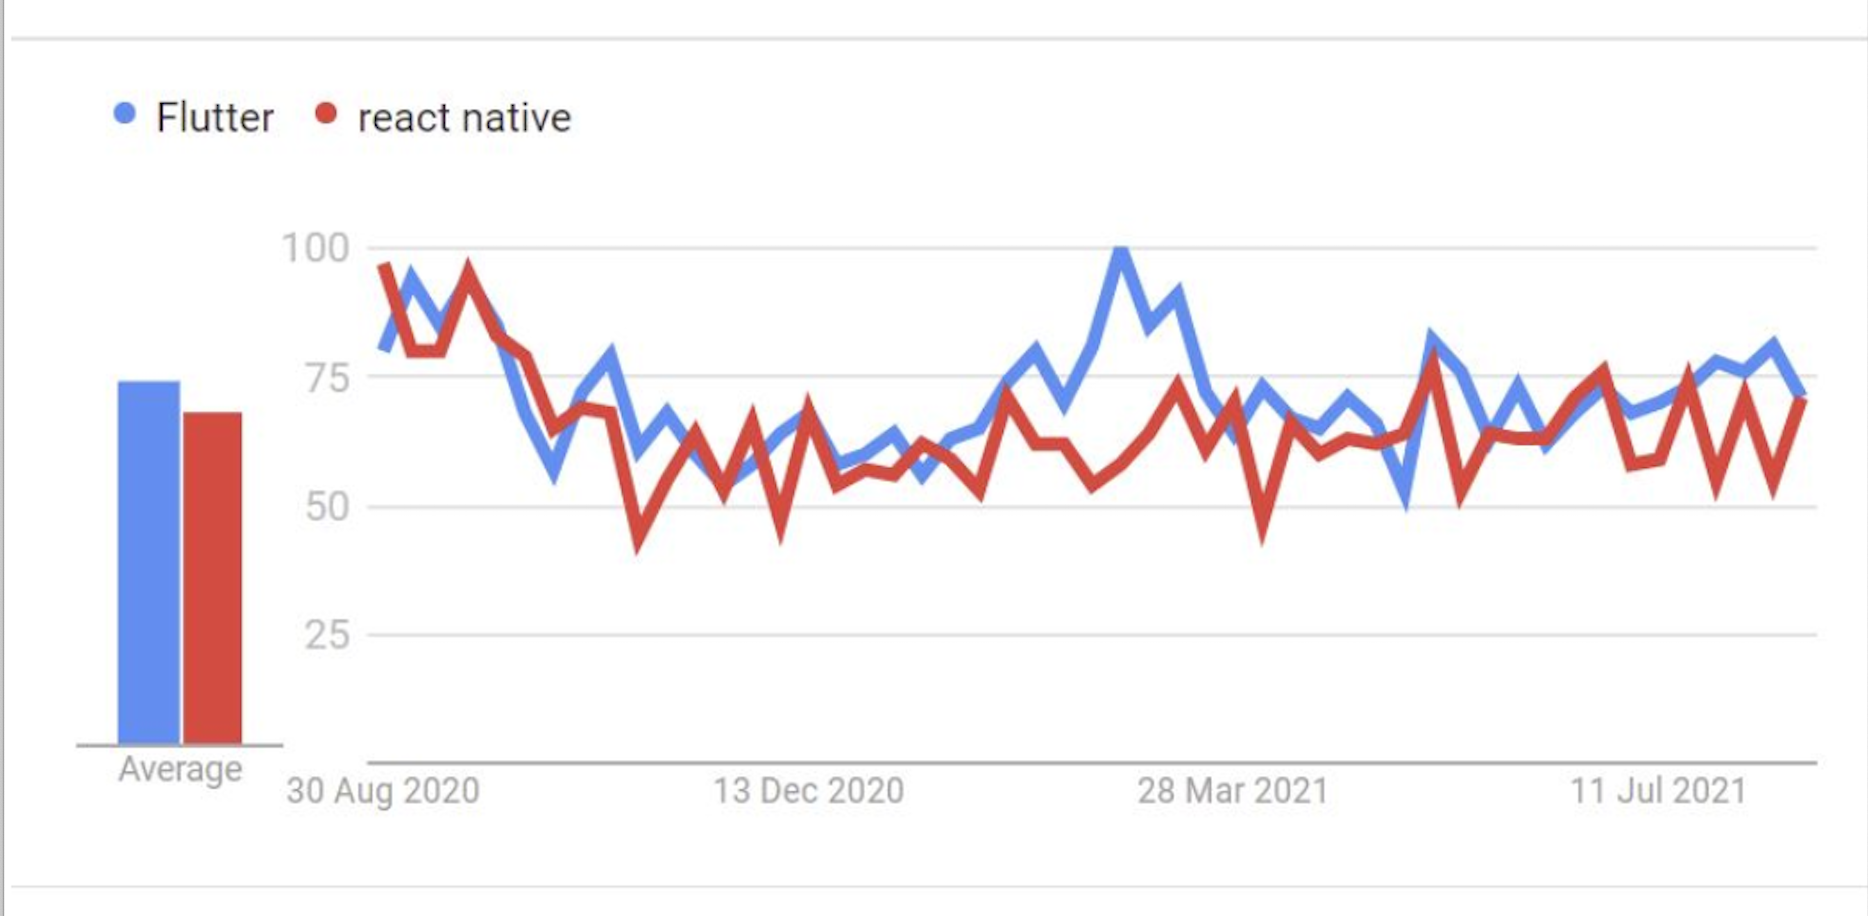
\includegraphics[width=0.9\textwidth]{images/reactNative_flutter.png}
        \caption{So sánh xu hướng tìm kiếm giữa Flutter và React Native \cite{goldenowlflutterreact}}
    \end{figure}

    Dưới đây là bảng so sánh một số khía cạnh chính giữa React Native và Flutter:

    \begin{table}[H]
        \centering
        \begin{tabular}{|l|p{3.5cm}|p{6cm}|}
            \hline
            \textbf{Tiêu chí} & \textbf{React Native} & \textbf{Flutter} \\
            \hline
            Ngôn ngữ lập trình & JavaScript (hoặc TypeScript) & Dart \\
            \hline
            Hiệu suất & Gần với native, phụ thuộc vào bridge & Cao hơn nhờ rendering engine riêng (Skia) \\
            \hline
            Giao diện người dùng & Dựa vào native components & Tùy chỉnh hoàn toàn, nhất quán mọi nền tảng \\
            \hline
            Cộng đồng & Lâu đời hơn, cộng đồng lớn & Đang phát triển nhanh chóng, được Google hỗ trợ mạnh \\
            \hline
            Tài liệu & Đầy đủ, nhiều ví dụ thực tiễn & Rõ ràng, cấu trúc tốt, phù hợp cho người mới bắt đầu \\
            \hline
        \end{tabular}
        \caption{So sánh các yếu tố giữa React Native và Flutter \cite{codetodeploy2025}}
    \end{table}

% 2.7
\subsection{Kết luận phần Cơ Sở Lý Thuyết}
\renewcommand{\labelitemi}{--}    
    
        Kiến trúc đa nền tảng đã phát triển qua nhiều giai đoạn, từ các giải pháp dựa trên WebView đến các framework hiện đại như React Native và Flutter. Mỗi công cụ có ưu nhược điểm riêng, phù hợp với từng loại dự án. Việc lựa chọn phụ thuộc vào sự cân nhắc giữa chi phí, thời gian, và chất lượng, cùng với định hướng dài hạn của doanh nghiệp. Xu hướng tương lai hứa hẹn sự tích hợp sâu rộng của AI, WebAssembly và low-code platforms, mở ra kỷ nguyên mới cho phát triển ứng dụng linh hoạt và hiệu quả.
\section{Phân Tích Các Framework}

  React Native và Flutter là hai framework đa nền tảng phổ biến, mỗi framework mang đến những ưu điểm và thách thức riêng. React Native, phát triển bởi Facebook, cho phép sử dụng JavaScript và tái sử dụng mã nguồn giữa các nền tảng iOS và Android, giúp tiết kiệm chi phí và thời gian phát triển. Với hệ sinh thái phong phú và cộng đồng lớn, React Native dễ dàng tích hợp với các công nghệ khác. Ngược lại, Flutter, do Google phát triển, sử dụng ngôn ngữ Dart và engine render riêng, giúp tối ưu hóa hiệu suất và tạo giao diện người dùng đẹp mắt, đồng thời mang lại hiệu quả cao trong việc phát triển ứng dụng yêu cầu đồ họa phức tạp. Tuy nhiên, Flutter còn thiếu sự phong phú của các plugin và thư viện như React Native. Việc lựa chọn giữa hai framework này phụ thuộc vào yêu cầu dự án, với React Native phù hợp cho các ứng dụng cần phát triển nhanh và dễ dàng tích hợp, còn Flutter thích hợp cho những ứng dụng yêu cầu hiệu suất và giao diện đặc biệt.

% 3.1
\subsection{React Native}
\renewcommand{\labelitemi}{--}    
\subsubsection{Kiến Trúc}

\begin{sloppypar}
React Native là một framework phát triển ứng dụng đa nền tảng do Meta (trước đây là Facebook) phát triển. Nó kết hợp giữa JavaScript và native code để xây dựng ứng dụng di động có giao diện mượt mà và khả năng mở rộng cao.
\end{sloppypar}

\vspace{0.5em}

\begin{sloppypar}
Kiến trúc của React Native bao gồm ba thành phần chính: \textbf{JavaScript VM}, \textbf{Bridge}, và \textbf{Native Modules}.
\end{sloppypar}

\vspace{0.5em}

\begin{figure}[H]
    \centering
    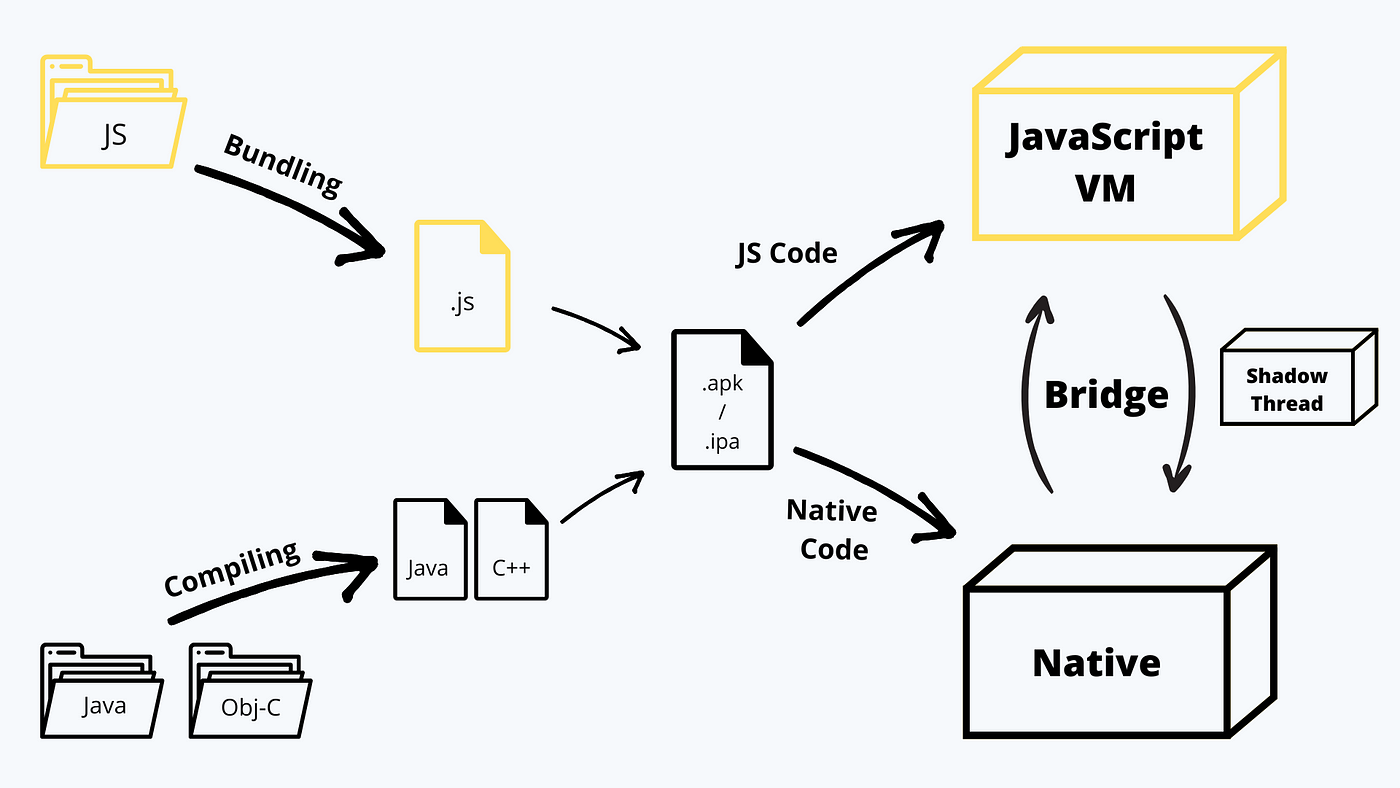
\includegraphics[width=0.95\textwidth]{images/react_native.png}
    \caption{Kiến trúc tổng quan của React Native~\cite{react-native-fabric}}
\end{figure}

\begin{sloppypar}
Trước tiên, JavaScript VM (Virtual Machine) là nơi thực thi logic nghiệp vụ của ứng dụng.  
Khi người dùng tương tác, các hàm JavaScript sẽ xử lý sự kiện, gọi API hoặc thao tác dữ liệu.  
Trên iOS, React Native sử dụng JavaScriptCore của WebKit; trên Android, Meta ưu tiên dùng Hermes – engine nhẹ giúp giảm thời gian khởi động 30\%.  
Ví dụ, Bloomberg đã sử dụng Hermes để tối ưu tốc độ cập nhật dữ liệu chứng khoán thời gian thực.
\end{sloppypar}

\vspace{0.5em}

\begin{sloppypar}
Tiếp theo, Native Modules là các thành phần được viết bằng ngôn ngữ nền tảng như Java/Kotlin hoặc Obj-C/Swift.  
Chúng cho phép ứng dụng truy cập các API hệ điều hành, ví dụ như GPS hoặc camera.  
Một ví dụ cụ thể là Walmart sử dụng Native Modules để tích hợp thanh toán NFC, đảm bảo hiệu suất và bảo mật cao.
\end{sloppypar}

\vspace{0.5em}

\begin{sloppypar}
Bridge đóng vai trò là cầu nối giữa JavaScript và native code.  
Khi JavaScript cần gọi chức năng nền tảng, Bridge sẽ truyền dữ liệu qua định dạng JSON – một quy trình tốn thời gian do phải serialize/\-deserialize.  
Theo Đại học Oslo (2022), việc giao tiếp này có thể gây trễ 5–15ms.  
Để khắc phục, Meta giới thiệu kiến trúc mới mang tên Fabric (2023), sử dụng JSI (JavaScript\- Interface) cho phép truy cập trực tiếp native code, giúp cải thiện tốc độ render đến 40\%.
\end{sloppypar}

\subsubsection{Ưu Điểm}
React Native mang lại nhiều lợi ích đáng kể, đặc biệt là khả năng tái sử dụng mã nguồn và tốc độ phát triển nhanh.

\vspace{0.5em}

Một trong những điểm mạnh lớn nhất là khả năng chia sẻ code giữa web và mobile. Ví dụ, Airbnb đã tái sử dụng đến 60\% codebase giữa hai nền tảng, tiết kiệm đáng kể thời gian phát triển. Thư viện \texttt{React Native Web} giúp chuyển đổi component React Native sang React DOM để chạy trên trình duyệt.

\vspace{0.5em}

Ngoài ra, hệ sinh thái npm khổng lồ (hơn 2.1 triệu package, 2023) giúp tăng tốc độ lập trình. Thư viện như \texttt{React Navigation} đơn giản hóa routing phức tạp, trong khi \texttt{React Native Maps} hỗ trợ hiển thị bản đồ chính xác.

\vspace{0.5em}

Cuối cùng, React Native cung cấp Live Reload và Hot Reload – hai công cụ giúp lập trình viên cập nhật UI ngay tức thì mà không mất trạng thái. Theo khảo sát của JetBrains (2022), tính năng này giúp rút ngắn thời gian debug đến 30\%.

\subsubsection{Nhược Điểm}

Dù có nhiều lợi ích, React Native vẫn tồn tại một số hạn chế nhất định, đặc biệt về hiệu năng và khả năng tùy biến.

\vspace{0.5em}

Do phụ thuộc vào Bridge, hiệu năng ứng dụng thấp hơn so với native. Ví dụ, render danh sách 1.000 phần tử trên React Native mất 320ms, trong khi native Android chỉ cần 210ms (Biorn-Hansen, 2021). Các ứng dụng yêu cầu đồ họa cao như game 3D hay video editor không phù hợp với React Native.

\vspace{0.5em}

Một vấn đề khác là phụ thuộc vào thư viện bên thứ ba. Khi nền tảng hệ điều hành thay đổi, các thư viện có thể không cập nhật kịp. Ví dụ, React Native Firebase gặp lỗi nghiêm trọng khi Android 13 thay đổi cơ chế cấp quyền, gây crash ứng dụng diện rộng.

\vspace{0.5em}

Cuối cùng, việc tùy chỉnh UI phức tạp như animation nâng cao hay tích hợp OpenGL đòi hỏi viết code native.  
Điều này làm tăng độ phức tạp và yêu cầu đội ngũ có kinh nghiệm phát triển native.

% 3.2
\subsection{Flutter}
\renewcommand{\labelitemi}{--}    
\subsubsection{Kiến Trúc}

Flutter là framework đa nền tảng do Google phát triển, sử dụng ngôn ngữ Dart và engine Skia để tự render giao diện người dùng, không phụ thuộc vào thành phần native.

\begin{figure}[H]
    \centering
    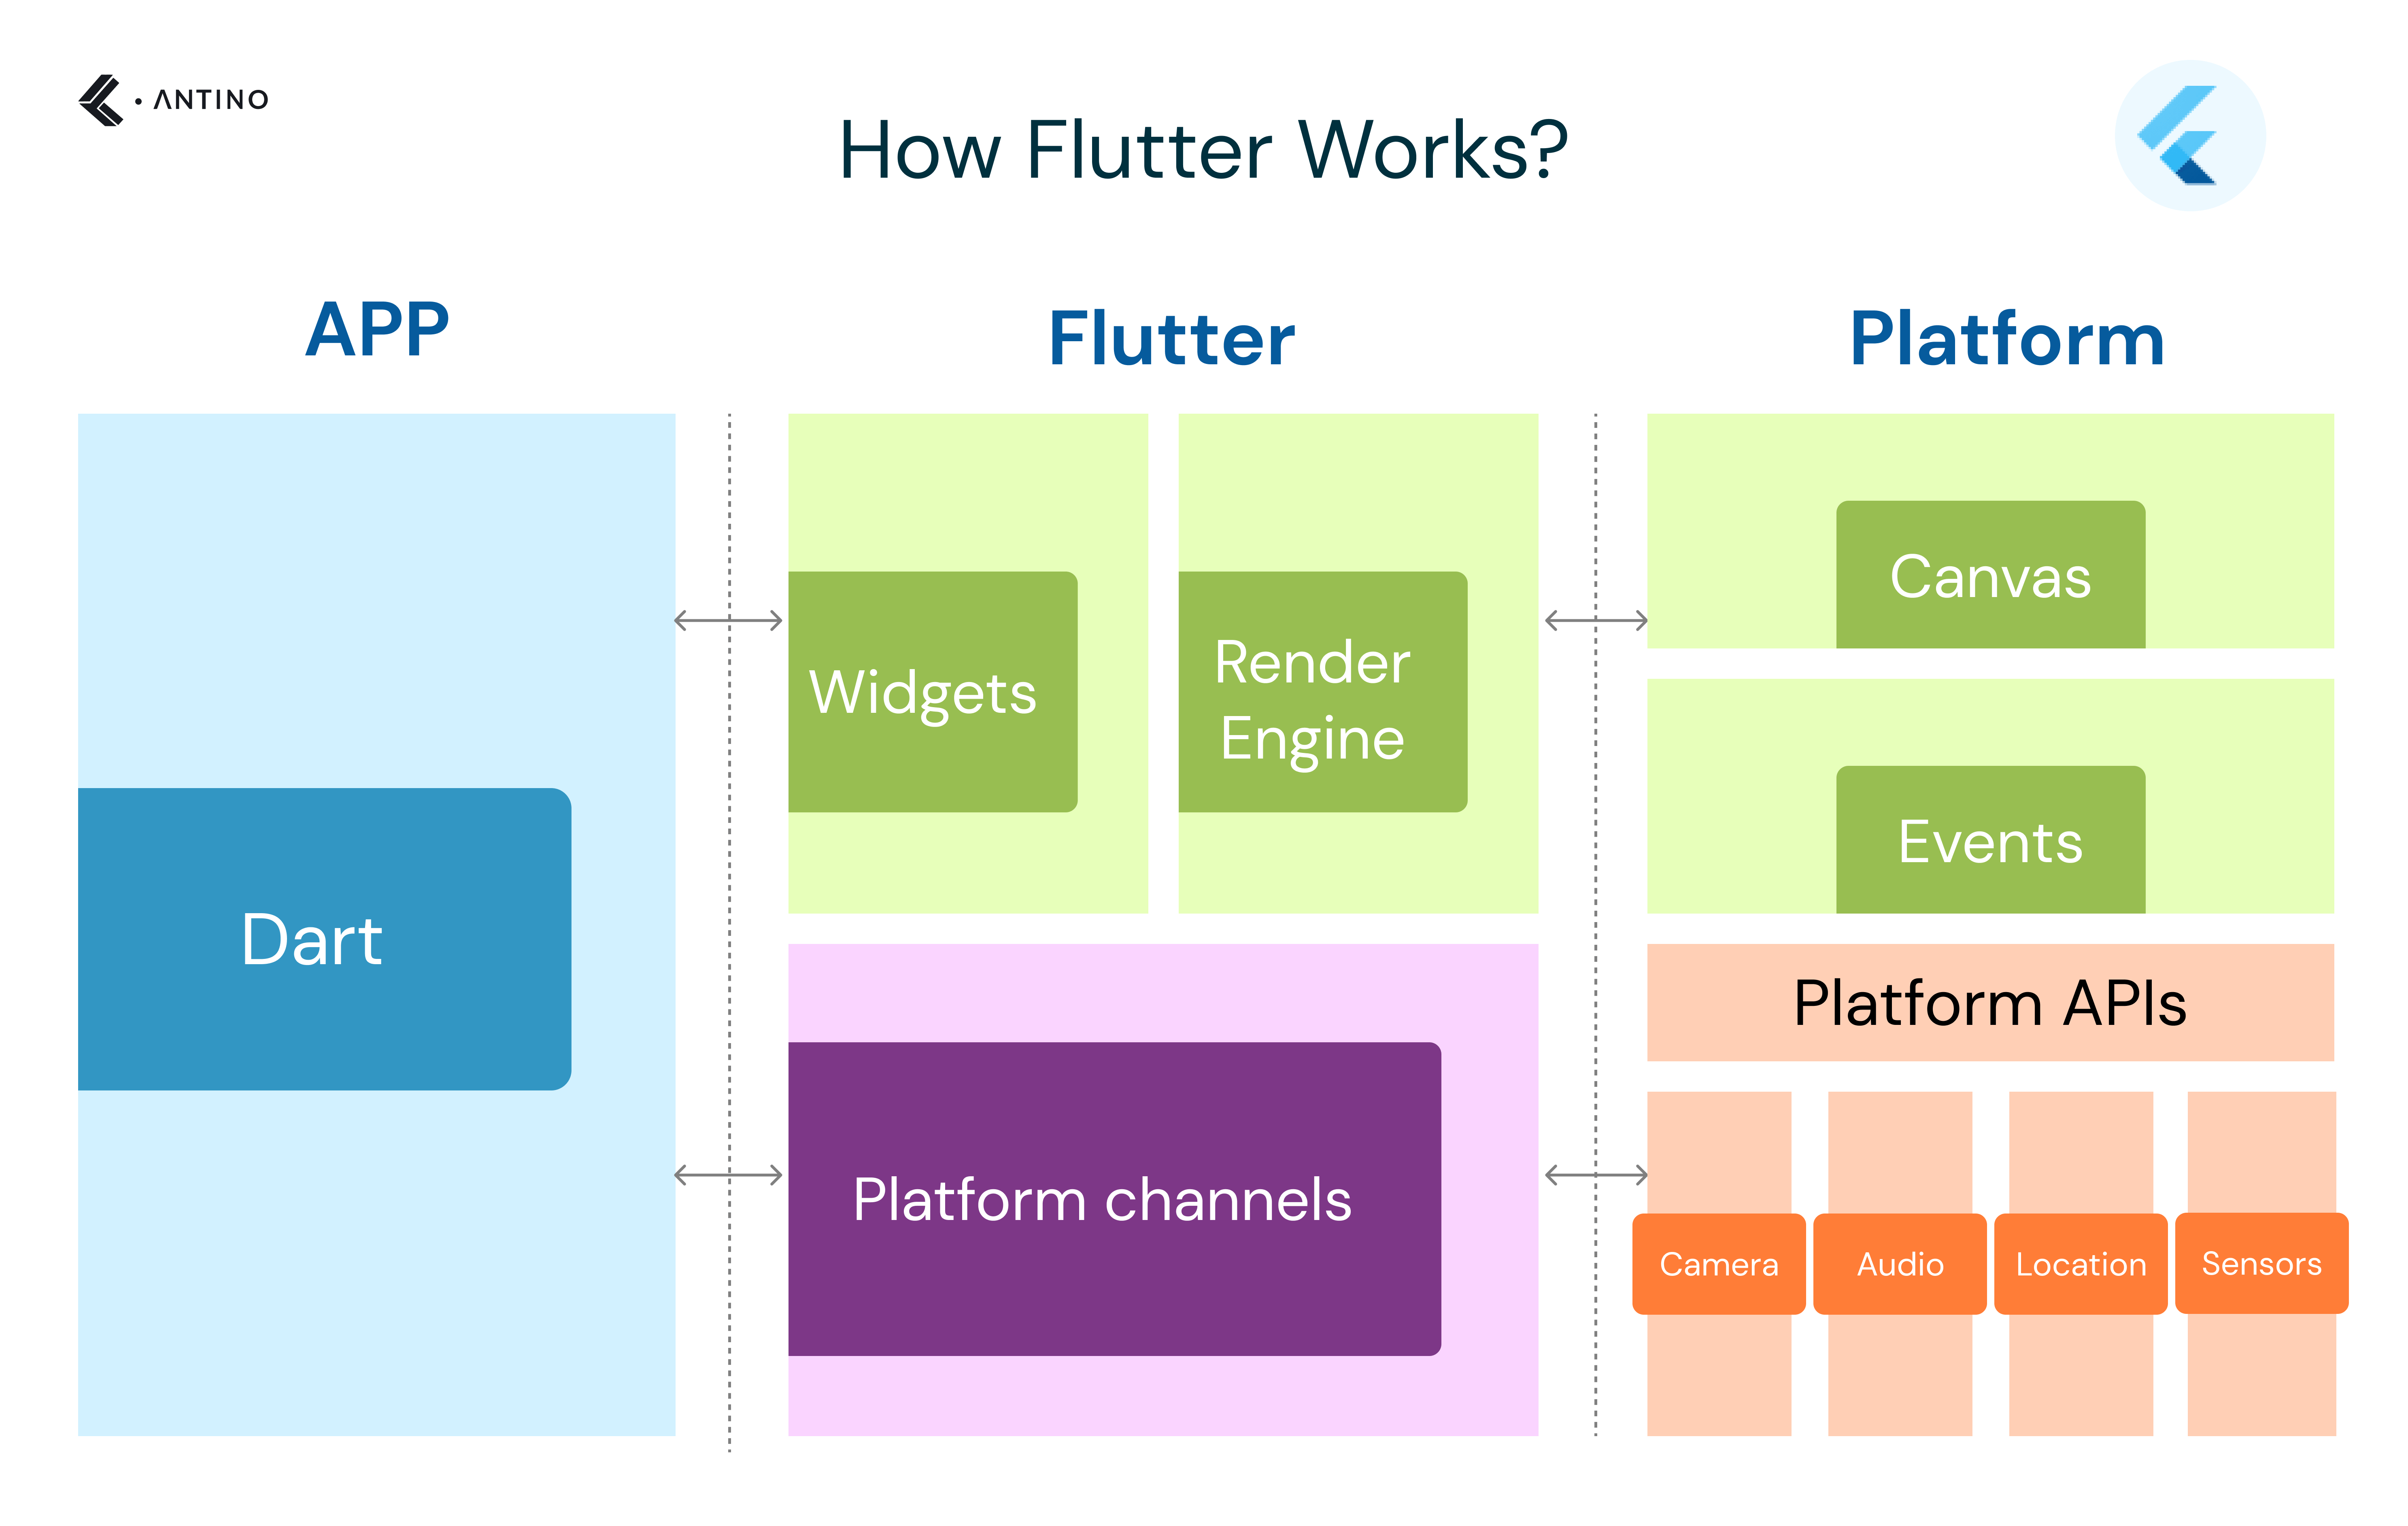
\includegraphics[width=0.75\textwidth]{images/flutter.png}
    \caption{Kiến trúc tổng quan của Flutter~\cite{flutter-impeller}}
\end{figure}

Dart là ngôn ngữ lập trình cốt lõi của Flutter, được thiết kế để kết hợp hiệu suất cao và tính linh hoạt. Dart hỗ trợ hai chế độ biên dịch: AOT (Ahead-of-Time) để tạo mã native tối ưu cho hiệu năng, và JIT (Just-in-Time) cho phép Hot Reload khi phát triển. Ví dụ, Alibaba đã dùng Dart để xử lý tới 50 triệu giao dịch/ngày, tận dụng khả năng xử lý bất đồng bộ hiệu quả với \texttt{Future}, \texttt{async/await}.

\vspace{0.5em}

Tiếp theo, engine Skia là thành phần chịu trách nhiệm vẽ toàn bộ UI lên một canvas duy nhất thay vì sử dụng native widgets. Điều này đảm bảo giao diện nhất quán trên mọi nền tảng. Chẳng hạn, nút \texttt{ElevatedButton} trong Flutter được render trực tiếp, cho phép tùy biến đến từng pixel. Ứng dụng như Starbucks hoặc eBay đã sử dụng Skia để đảm bảo tính thương hiệu trên iOS và Android đồng nhất.

\vspace{0.5em}

Flutter tổ chức UI theo mô hình widget – mọi thành phần đều là widget, kể cả layout và animation.  
Có hai loại chính:
\begin{itemize}
    \item \textbf{StatelessWidget}: không thay đổi trạng thái (ví dụ: văn bản tĩnh, biểu tượng).
    \item \textbf{StatefulWidget}: có thể thay đổi theo thời gian hoặc tương tác (ví dụ: checkbox, form).
\end{itemize}

Ngoài ra, Flutter hỗ trợ hai thư viện giao diện: \texttt{Material} (Google style) và \texttt{Cupertino} (iOS style), cho phép tạo trải nghiệm quen thuộc tùy theo nền tảng.

\vspace{0.5em}

Flutter giao tiếp với native thông qua \textbf{Platform Channels}, cho phép gọi các hàm nền tảng như GPS, camera hoặc Bluetooth.  
Ví dụ, khi ứng dụng cần truy cập cảm biến gia tốc, Flutter sẽ gửi message qua channel và native sẽ trả về dữ liệu tương ứng.

\subsubsection{Ưu Điểm}

Flutter nổi bật nhờ hiệu năng cao và khả năng tùy chỉnh mạnh:

\vspace{0.5em}

Thứ nhất, Flutter có hiệu năng gần như native nhờ sử dụng AOT compilation.  
Các ứng dụng như Google Pay đạt 60 FPS ngay cả trên thiết bị cấu hình thấp, với độ trễ phản hồi giao dịch dưới 100ms.

\vspace{0.5em}

Thứ hai, tính năng \textbf{Hot Reload} cho phép lập trình viên cập nhật giao diện tức thì mà không mất trạng thái ứng dụng.  
Theo báo cáo từ BMW, tính năng này đã giúp nhóm thiết kế UI giảm tới 50\% thời gian phát triển.

\vspace{0.5em}

Thứ ba, Flutter hỗ trợ đa nền tảng từ một codebase duy nhất, bao gồm Android, iOS, web, Windows, macOS và Linux. Ví dụ, ứng dụng Reflectly đạt 95\% tái sử dụng mã nguồn, giúp giảm 70\% chi phí bảo trì so với phát triển riêng lẻ từng nền tảng.

\subsubsection{Nhược Điểm}

Mặc dù có nhiều ưu điểm, Flutter vẫn còn một số hạn chế kỹ thuật đáng lưu ý:

\vspace{0.5em}

Đầu tiên, kích thước ứng dụng Flutter tương đối lớn.  
Một ứng dụng Flutter trống có thể lên đến 20MB, do nhúng sẵn Dart runtime và Skia engine – lớn hơn nhiều so với React Native (khoảng 4MB).  
Điều này ảnh hưởng đến người dùng ở khu vực có tốc độ Internet chậm.

\vspace{0.5em}

Tiếp theo, lập trình viên phải học ngôn ngữ Dart – vốn chưa phổ biến như JavaScript. Cú pháp Dart tương đối mới với nhiều người, đặc biệt trong xử lý bất đồng bộ sử dụng \texttt{Future}, \texttt{Stream} thay vì \texttt{Promise} như trong JS.

\vspace{0.5em}

Cuối cùng, hệ sinh thái thư viện của Flutter nhỏ hơn React Native. Tính đến 2023, Flutter có khoảng 25.000 package trên pub.dev, so với hơn 50.000 package của React Native trên npm. Điều này khiến việc tìm thư viện phù hợp đôi khi gặp hạn chế, đặc biệt với các chức năng phức tạp hoặc mới xuất hiện.

% 3.3
\subsection{So sánh React Native và Flutter}
\renewcommand{\labelitemi}{--}

\subsubsection{Hiệu năng khi cuộn (Scrolling)}

  Theo biểu đồ Figure~\ref{fig:scrolling}, Flutter duy trì tốc độ khung hình ổn định gần 60 FPS trong khi React Native có hiện tượng drop mạnh xuống dưới 30 FPS do độ trễ từ bridge giữa UI thread và JavaScript thread. Điều này cho thấy Flutter có hiệu năng cuộn mượt mà hơn, thích hợp với các ứng dụng có nhiều tương tác như game hoặc trình chỉnh sửa ảnh.

\begin{figure}[H]
    \centering
    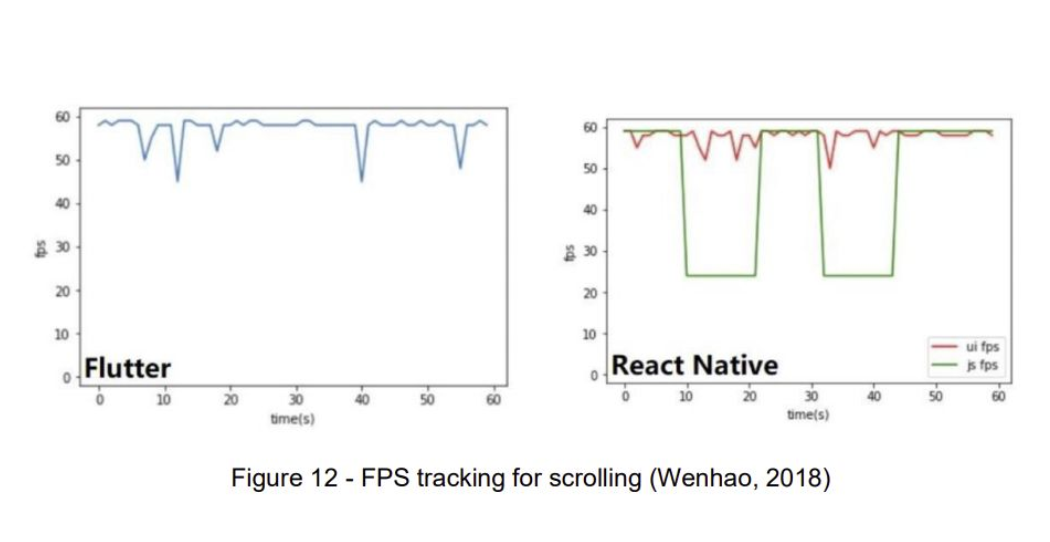
\includegraphics[width=0.8\linewidth]{images/scrolling.png}
    \caption{FPS khi cuộn của Flutter và React Native (Wenhao, 2018)}
    \label{fig:scrolling}
\end{figure}

\subsubsection{Ghi dữ liệu (Write Performance)}

  Biểu đồ Figure~\ref{fig:write} cho thấy thời gian ghi đơn lẻ và trung bình của React Native thấp hơn Flutter, phản ánh hiệu suất tốt hơn ở tác vụ ghi nhẹ. Tuy nhiên, chênh lệch không quá lớn và có thể không đáng kể trong hầu hết ứng dụng thực tế.

\begin{figure}[H]
    \centering
    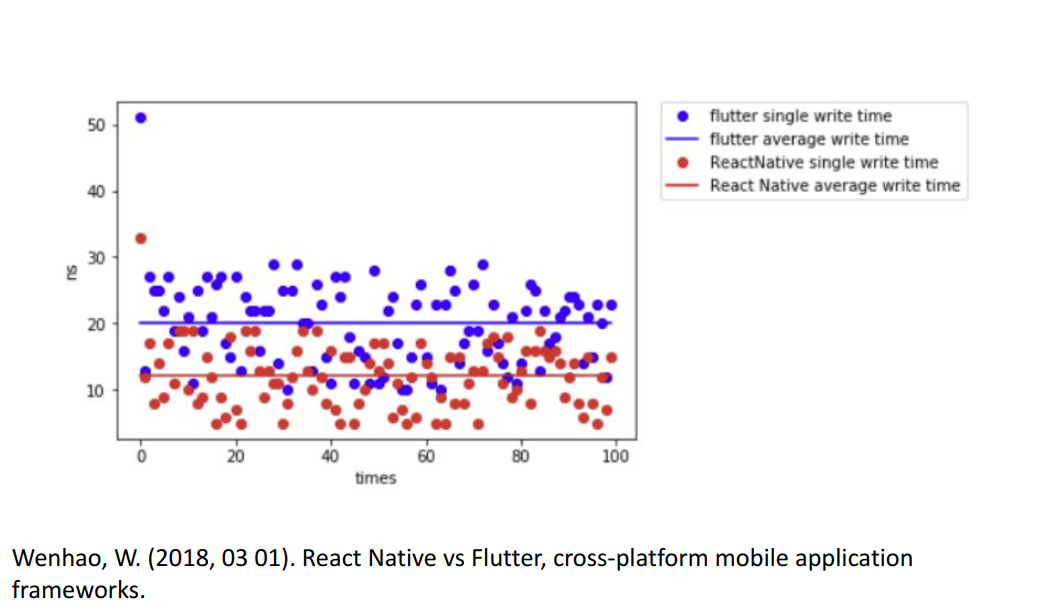
\includegraphics[width=0.8\linewidth]{images/read_write.png}
    \caption{Hiệu suất ghi dữ liệu của Flutter và React Native (Wenhao, 2018)}
    \label{fig:write}
\end{figure}

\subsubsection{Hiệu năng tổng thể theo nghiên cứu mới nhất}

  Theo Biorn-Hansen (2021), React Native và Flutter có điểm tổng thể thấp hơn Native, MAML/MD\textsuperscript{2} và NativeScript về hiệu năng cầu nối (bridge performance). Flutter đạt tổng điểm 15, thấp hơn React Native (16), chủ yếu do sử dụng nhiều RAM tính toán hơn. Tuy nhiên, Flutter vẫn là lựa chọn đáng cân nhắc nếu hiệu năng hình ảnh (UI performance) là yếu tố ưu tiên.

\begin{figure}[H]
    \centering
    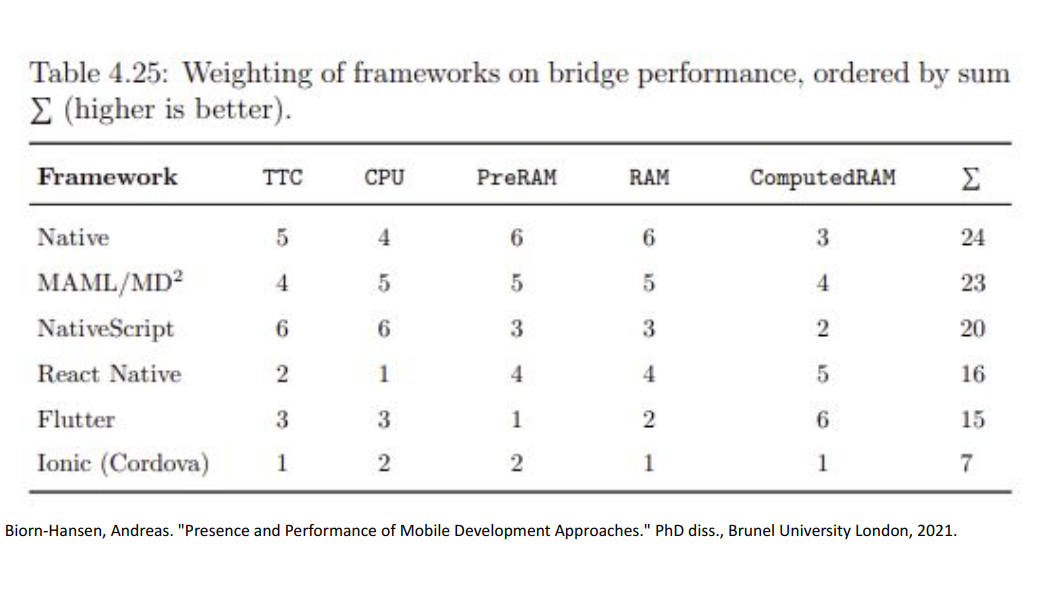
\includegraphics[width=0.7\linewidth]{images/performance.png}
    \caption{Đánh giá hiệu năng framework theo Biorn-Hansen (2021)}
    \label{fig:overall}
\end{figure}

\subsubsection{Ngôn ngữ lập trình}

  React Native sử dụng JavaScript – một ngôn ngữ phổ biến, dễ học, hỗ trợ từ hệ sinh thái Node.js và thư viện lớn. Trong khi đó, Flutter dùng Dart – một ngôn ngữ được Google phát triển với ưu điểm về type safety và khả năng biên dịch AOT, giúp giảm lỗi runtime nhưng đòi hỏi thời gian làm quen.

\subsubsection{Phát triển đa nền tảng}

  React Native chủ yếu nhắm đến iOS và Android, tuy có hỗ trợ web nhưng chưa ổn định. Ngược lại, Flutter hỗ trợ 6 nền tảng gồm mobile, web và desktop (Windows, macOS, Linux), phù hợp với ứng dụng cần độ bao phủ rộng và giao diện đồng nhất.

\subsubsection{Cộng đồng và tài nguyên}

  React Native sở hữu cộng đồng lớn với hơn 2 triệu developer, tài nguyên phong phú trên Stack Overflow, GitHub và blog kỹ thuật. Flutter tuy mới hơn nhưng đang tăng trưởng nhanh, đặc biệt ở thị trường châu Á, được Google đầu tư mạnh về tài liệu và hỗ trợ chính thức.

% 3.4
\subsection{Case Study}
\renewcommand{\labelitemi}{--}    
\subsubsection{React Native: Instagram}

  Instagram đã tích hợp React Native vào ứng dụng native hiện có nhằm tăng tốc độ phát triển các tính năng như \textit{Stories} và giao diện máy ảnh (\textit{Camera UI}). Một trong những thách thức chính là đảm bảo hiệu năng ổn định trên các thiết bị cũ như iPhone 6s. Đội ngũ phát triển đã áp dụng kỹ thuật \textit{lazy loading} để tải component khi cần thiết và tối ưu cầu nối (\textit{bridge}) bằng cách giảm thiểu số lần tương tác giữa JavaScript và native thread. Kết quả, họ tái sử dụng được khoảng 85\% mã nguồn giữa hai nền tảng iOS và Android, đồng thời rút ngắn 30\% thời gian phát triển tính năng.

\subsubsection{Flutter: Google Ads}

  Ứng dụng Google Ads được xây dựng bằng Flutter nhằm hỗ trợ quản lý quảng cáo trên nhiều nền tảng. Ứng dụng này xử lý trung bình 5 triệu request mỗi ngày từ 16 quốc gia, với yêu cầu độ trễ phản hồi không vượt quá 200ms. Nhóm phát triển đã tận dụng \textit{Dart isolates} để thực hiện các tác vụ tính toán nặng ở luồng phụ, kết hợp với Firebase để đồng bộ dữ liệu thời gian thực (\textit{real-time}). Kết quả là thời gian tải dữ liệu giảm 40\%, đồng thời giao diện người dùng duy trì tốc độ khung hình 60 FPS trên tất cả thiết bị, bao gồm cả thiết bị cấu hình thấp.

% 3.5
\subsection{Kết Luận}
\renewcommand{\labelitemi}{--}    

  Cả React Native và Flutter đều là những framework hàng đầu cho phát triển ứng dụng đa nền tảng. Tuy nhiên, mỗi công nghệ lại phù hợp với những mục tiêu và điều kiện cụ thể trong quá trình phát triển.
  
  \setlength{\leftmargini}{1.5cm}
  \begin{itemize}
    \item Đối với các startup mong muốn đưa sản phẩm ra thị trường nhanh chóng, React Native là lựa chọn lý tưởng nhờ khả năng tái sử dụng mã JavaScript và cộng đồng phát triển rộng lớn.
    \item Trong khi đó, Flutter thể hiện ưu thế vượt trội ở những dự án yêu cầu hiệu năng cao và giao diện người dùng tuỳ chỉnh phức tạp nhờ engine đồ hoạ tích hợp và khả năng biên dịch trực tiếp sang mã máy.
  \end{itemize}
\vspace{0.5em}


  Trong tương lai, cả hai framework đều đang theo đuổi các hướng phát triển mới nhằm mở rộng phạm vi ứng dụng.

  \setlength{\leftmargini}{1.5cm}
  \begin{itemize}
    \item Flutter được kỳ vọng sẽ mở rộng sang các hệ thống nhúng như thiết bị IoT hoặc ô tô thông minh, đặc biệt thông qua dự án Hummingbird.
    \item Ngược lại, React Native đang tập trung vào cải thiện hiệu năng lõi bằng các sáng kiến như Fabric và TurboModules, giúp tối ưu giao tiếp giữa native và JavaScript.
  \end{itemize}
\vspace{0.5em}


  Việc lựa chọn framework phù hợp nên dựa trên các tiêu chí rõ ràng về kỹ thuật và nguồn lực.

  \setlength{\leftmargini}{1.5cm}
  \begin{itemize}
    \item Trước khi quyết định, nhóm phát triển nên đánh giá yêu cầu về giao diện, hiệu năng, cũng như kỹ năng sẵn có trong đội ngũ.
    \item Bên cạnh đó, việc xây dựng nguyên mẫu (\textit{prototype}) bằng cả hai công nghệ để kiểm thử hiệu suất thực tế là cách tiếp cận thực tiễn và hiệu quả.
  \end{itemize}

\section{Phân tích chi tiết các kiến trúc phần mềm}

% 
\subsection{Kiến trúc phần mềm ba tầng (Three-tier architecture)}
\renewcommand{\labelitemi}{--}    
    \begin{flushleft}
        \hspace*{0.8cm}Đây là một mô hình tổ chức phần mềm phổ biến, đặc biệt phù hợp với các hệ thống lớn, có khả năng mở rộng và bảo trì lâu dài. Mô hình này phân chia rõ ràng trách nhiệm của từng tầng, từ việc hiển thị, xử lý logic cho đến lưu trữ dữ liệu. Việc áp dụng kiến trúc ba tầng giúp ứng dụng dễ bảo trì, linh hoạt trong mở rộng và tăng khả năng tái sử dụng mã nguồn.
    \end{flushleft}

    \begin{flushleft}
      \hspace*{0.8cm}Kiến trúc ba tầng có thể áp dụng cho nhiều loại ứng dụng khác nhau: từ ứng dụng đơn giản đến phức tạp, từ ứng dụng độc lập đến ứng dụng kết nối mạng. Việc tách biệt ba tầng không chỉ làm cho mã nguồn trở nên rõ ràng hơn mà còn cho phép các nhóm phát triển làm việc độc lập trên từng tầng.
    \end{flushleft}

    \begin{flushleft}
      \hspace*{0.8cm}Tầng trình diễn (Presentation Layer), đây là tầng giao tiếp với người dùng. Chức năng chính của tầng này bao gồm:
      \setlength{\leftmargini}{1.5cm}
      \begin{itemize}
          \item Hiển thị dữ liệu từ tầng nghiệp vụ theo giao diện trực quan.
          \item Nhận lệnh từ người dùng (qua các nút bấm, form, tương tác giao diện).
          \item Không xử lý logic nghiệp vụ, nhờ vậy giao diện có thể dễ dàng tái sử dụng, thay đổi hoặc cập nhật mà không ảnh hưởng đến các tầng khác.
          \item[]$\Rightarrow$ Một lợi ích lớn là khả năng “lắp ghép” lại với các tầng nghiệp vụ khác nhau – giúp cùng một giao diện có thể sử dụng cho nhiều phiên bản khác nhau của hệ thống.
      \end{itemize}
    \end{flushleft}

    \begin{flushleft}
      \hspace*{0.8cm}Tầng nghiệp vụ (Business Logic Layer), tầng này giữ vai trò trung tâm trong hệ thống. Nó thực hiện:
      \setlength{\leftmargini}{1.5cm}
      \begin{itemize}
          \item Chuẩn bị dữ liệu đầu vào để gửi đến tầng dữ liệu.
          \item Chuyển đổi, xử lý dữ liệu nhận về để trả lại cho tầng trình diễn.
          \item Xử lý các lỗi logic hoặc lỗi phản hồi từ tầng dữ liệu.
          \item Áp dụng các quy tắc nghiệp vụ, như kiểm tra hợp lệ, xử lý quy trình.
          \item[]$\Rightarrow$ Tầng này giúp cô lập các xử lý phức tạp khỏi giao diện và dữ liệu, đảm bảo khả năng kiểm thử và bảo trì cao.
      \end{itemize}
    \end{flushleft}

    \begin{flushleft}
      \hspace*{0.8cm}Tầng dữ liệu (Data Layer), là nơi lưu trữ các thông tin quan trọng nhất của ứng dụng:
      \setlength{\leftmargini}{1.5cm}
      \begin{itemize}
          \item Lưu trữ cơ sở dữ liệu (SQL, NoSQL…).
          \item Thực hiện các truy vấn để đảm bảo hiệu năng và độ chính xác cao.
          \item Có thể tích hợp với cơ sở dữ liệu từ xa (server), hệ thống lưu trữ đám mây hoặc tệp cục bộ.
          \item[]$\Rightarrow$ Việc tối ưu tầng dữ liệu giúp cải thiện đáng kể hiệu năng của toàn hệ thống, đặc biệt là trong các ứng dụng có lượng dữ liệu lớn.
      \end{itemize}
    \end{flushleft}

    \begin{flushleft}
      \hspace*{0.8cm}$\Rightarrow$ Kiến trúc ba tầng mang lại lợi ích lớn về mặt tổ chức mã nguồn, bảo trì, kiểm thử và phát triển theo nhóm. Mỗi tầng có trách nhiệm riêng, từ đó giúp ứng dụng dễ mở rộng và thích ứng với thay đổi trong tương lai.
    \end{flushleft}

% 4.2
\subsection{Kiến trúc MVC (Model – View – Controller)}
\renewcommand{\labelitemi}{--}    
    \begin{flushleft}
        \hspace*{0.8cm}MVC (Model – View – Controller) là một mẫu kiến trúc phần mềm cổ điển, phổ biến trong phát triển ứng dụng, đặc biệt là trên nền tảng iOS. Mục tiêu chính của kiến trúc MVC là tách biệt rõ ràng giữa dữ liệu, giao diện và điều khiển xử lý, từ đó giúp ứng dụng dễ bảo trì, mở rộng và nâng cao trải nghiệm người dùng.
    \end{flushleft}

    \begin{flushleft}
      \hspace*{0.8cm}Mô hình này được hình dung như một sơ đồ ba thành phần, mỗi thành phần đảm nhận một vai trò cụ thể:
      \setlength{\leftmargini}{1.5cm}
      \begin{itemize}
          \item Model: Dữ liệu và logic xử lý dữ liệu.
          \item View: Giao diện hiển thị cho người dùng.
          \item Controller: Bộ điều phối, tiếp nhận hành động từ người dùng và điều khiển luồng xử lý.
          \item[]$\Rightarrow$ Ba thành phần hoạt động tách biệt nhưng liên kết chặt chẽ, đảm bảo ứng dụng vận hành trơn tru và dễ dàng điều chỉnh một phần mà không ảnh hưởng đến phần còn lại.
      \end{itemize}
    \end{flushleft}

    \begin{flushleft}
      \hspace*{0.8cm}Model – Mô hình dữ liệu:
      \setlength{\leftmargini}{1.5cm}
      \begin{itemize}
          \item Định danh những gì cần trả về cho người dùng.
          \item Đây là nơi chứa dữ liệu thô, các quy tắc nghiệp vụ và các thao tác xử lý dữ liệu.
          \item Ví dụ: trong một ứng dụng bán hàng, Model chứa thông tin sản phẩm, đơn hàng, người dùng...
      \end{itemize}
    \end{flushleft}

    \begin{flushleft}
      \hspace*{0.8cm}Controller – Bộ điều khiển:
      \setlength{\leftmargini}{1.5cm}
      \begin{itemize}
          \item Tiếp nhận các yêu cầu từ người dùng (qua View).
          \item Thực hiện các truy vấn tài nguyên, gọi các phương thức xử lý trong Model.
          \item Là “bộ não” điều phối mọi hoạt động trong ứng dụng.
      \end{itemize}
    \end{flushleft}

    \begin{flushleft}
      \hspace*{0.8cm}View – Giao diện người dùng:
      \setlength{\leftmargini}{1.5cm}
      \begin{itemize}
          \item Hiển thị dữ liệu dưới dạng dễ hiểu, thân thiện với người dùng.
          \item View không xử lý logic nghiệp vụ, mà chỉ phản hồi lại theo những gì Controller và Model cung cấp.
          \item View sẽ cập nhật nội dung mỗi khi Model thay đổi.
      \end{itemize}
    \end{flushleft}

    \begin{flushleft}
      \hspace*{0.8cm}MVC giúp tách biệt rõ ràng chức năng, dễ dàng phát triển, kiểm thử và bảo trì. Đồng thời cho phép nhiều lập trình viên làm việc song song: người thiết kế giao diện làm View, lập trình viên backend làm Model, còn Controller kết nối hai phần này. Ngoài ra, nó còn có tính tái sử dụng mã nguồn tốt khi một Model có thể được dùng cho nhiều View khác nhau.
    \end{flushleft}

    \begin{flushleft}
      \hspace*{0.8cm}$\Rightarrow$ Mẫu kiến trúc MVC là một giải pháp hiệu quả giúp tổ chức ứng dụng một cách khoa học và linh hoạt. Việc phân chia ứng dụng thành ba thành phần rõ ràng giúp giảm độ phức tạp khi mở rộng, dễ bảo trì, đồng thời nâng cao hiệu quả làm việc nhóm trong quá trình phát triển ứng dụng. Với iOS, MVC vẫn là lựa chọn được ưa chuộng và hỗ trợ tốt trong môi trường phát triển Xcode và Swift.
    \end{flushleft}

% 4.3
\subsection{Kiến trúc MVVM (Model - View - ViewModel)}
\renewcommand{\labelitemi}{--}    
    \begin{flushleft}
        \hspace*{0.8cm}Kiến trúc MVVM (Model – View – ViewModel) là một trong những mẫu thiết kế hiện đại, được áp dụng phổ biến trong phát triển ứng dụng Android (đặc biệt là với sự hỗ trợ từ Jetpack và Kotlin). MVVM ra đời nhằm tối ưu quá trình phát triển ứng dụng bằng cách tách biệt logic hiển thị và logic xử lý, đồng thời tăng tính tự động hóa trong việc cập nhật dữ liệu nhờ cơ chế Data Binding.
    \end{flushleft}

    \begin{flushleft}
      \hspace*{0.8cm}MVVM có cấu trúc gần giống với MVC, nhưng thay vì để Controller điều khiển toàn bộ luồng xử lý, MVVM đưa vào một tầng trung gian là ViewModel – chịu trách nhiệm “kết nối thông minh” giữa dữ liệu (Model) và giao diện (View):
      \setlength{\leftmargini}{1.5cm}
      \begin{itemize}
          \item Tương tự như MVC, View hiển thị dữ liệu, Model chứa dữ liệu và logic xử lý.
          \item Tuy nhiên, Controller được thay thế bằng ViewModel, giúp giảm bớt sự ràng buộc giữa View và Model.
      \end{itemize}
    \end{flushleft}

    \begin{flushleft}
      \hspace*{0.8cm}Model – Dữ liệu và logic xử lý:
      \setlength{\leftmargini}{1.5cm}
      \begin{itemize}
          \item Là nơi lưu trữ các dữ liệu chính của ứng dụng (như thông tin người dùng, sản phẩm...).
          \item Xử lý các nghiệp vụ như tính toán, truy xuất dữ liệu từ cơ sở dữ liệu hoặc API.
          \item Model không trực tiếp liên hệ với View, mà thông qua ViewModel.
      \end{itemize}
    \end{flushleft}

    \begin{flushleft}
      \hspace*{0.8cm}View – Giao diện hiển thị:
      \setlength{\leftmargini}{1.5cm}
      \begin{itemize}
          \item Là phần người dùng tương tác trực tiếp (giao diện ứng dụng).
          \item View trong MVVM không xử lý logic nghiệp vụ mà chỉ phản ánh lại các dữ liệu từ ViewModel.
          \item Nhờ vào Data Binding, View có thể tự động cập nhật khi dữ liệu trong ViewModel thay đổi – giúp giảm mã lặp và tăng hiệu suất phát triển.
      \end{itemize}
    \end{flushleft}

    \begin{flushleft}
      \hspace*{0.8cm}ViewModel – Cầu nối thông minh:
      \setlength{\leftmargini}{1.5cm}
      \begin{itemize}
          \item Chứa các Model và chuẩn bị dữ liệu để hiển thị cho View.
          \item Tạo ra các LiveData hoặc Observable để View có thể theo dõi và tự động cập nhật giao diện khi dữ liệu thay đổi.
          \item Đồng thời, ViewModel cũng xử lý việc truyền dữ liệu từ View sang Model, giúp cập nhật ngược lại khi người dùng nhập liệu hoặc thực hiện thao tác.
      \end{itemize}
    \end{flushleft}

    \begin{flushleft}
      \hspace*{0.8cm}Một điểm mạnh nổi bật của MVVM là cơ chế Data Binding – liên kết dữ liệu hai chiều:
      \setlength{\leftmargini}{1.5cm}
      \begin{itemize}
          \item Khi một đối tượng thuộc nhóm View (như EditText) thay đổi, dữ liệu tương ứng trong ViewModel (hoặc Model) cũng tự động cập nhật.
          \item Ngược lại, khi ViewModel thay đổi giá trị, View cũng cập nhật lại ngay lập tức.
          \item[]$\Rightarrow$ Điều này giúp hạn chế lỗi khi cập nhật giao diện và rút ngắn thời gian phát triển, đặc biệt là trong các ứng dụng có nhiều thao tác tương tác dữ liệu.
      \end{itemize}
    \end{flushleft}

    \begin{flushleft}
      \hspace*{0.8cm}$\Rightarrow$ MVVM là một mô hình kiến trúc mạnh mẽ, phù hợp với các ứng dụng hiện đại cần cập nhật giao diện linh hoạt, liên tục. Với sự hỗ trợ từ Data Binding và LiveData (trong Android), ViewModel giúp đơn giản hóa việc xử lý dữ liệu và đồng bộ giao diện, đồng thời giảm sự phụ thuộc giữa các thành phần, nâng cao khả năng bảo trì và mở rộng về sau. MVVM hiện là lựa chọn ưu tiên trong các dự án Android có quy mô từ vừa đến lớn.
    \end{flushleft}

% 4.4
\subsection{Kiến trúc Client/Server}
\renewcommand{\labelitemi}{--}    
    \begin{flushleft}
        \hspace*{0.8cm}Trong thời đại số, đa số các ứng dụng cần trao đổi dữ liệu qua Internet. Mô hình Client/Server trở thành kiến trúc không thể thiếu, đặc biệt với các ứng dụng có tính năng đồng bộ dữ liệu, chia sẻ thông tin theo thời gian thực, hoặc sử dụng tài nguyên trên máy chủ từ xa. Đồng thời, cần kết hợp với các kiến trúc nội bộ như MVC hoặc MVVM để tối ưu hóa việc xây dựng giao diện và xử lý logic.
    \end{flushleft}

    \begin{flushleft}
      \hspace*{0.8cm}Kiến trúc Client/Server mô tả mô hình trong đó ứng dụng Client (thiết bị người dùng) gửi yêu cầu đến Server (máy chủ từ xa), thường qua HTTP Request, WebSocket, hoặc Web Service. Các chức năng chính bao gồm:
      \setlength{\leftmargini}{1.5cm}
      \begin{itemize}
          \item Client: Gửi yêu cầu (request), hiển thị dữ liệu, tương tác với người dùng.
          \item Server: Xử lý yêu cầu, truy cập cơ sở dữ liệu, trả về dữ liệu kết quả.
          \item[]$\Rightarrow$ Kiến trúc này phù hợp cho các ứng dụng có nhiều người dùng, cần chia sẻ dữ liệu như mạng xã hội, ứng dụng ngân hàng, thương mại điện tử…
      \end{itemize}
    \end{flushleft}
\section{Cân Nhắc Khi Phát Triển}


  Khi lựa chọn giữa Flutter và React Native để phát triển ứng dụng di động, các yếu tố kỹ thuật, kinh tế và trải nghiệm người dùng cần được phân tích kỹ lưỡng. Dưới đây là chi tiết từng khía cạnh để hỗ trợ quyết định.

% 5.1
\subsection{Yếu tố kỹ thuật}

Yếu tố kỹ thuật đóng vai trò cốt lõi trong việc đảm bảo ứng dụng hoạt động ổn định, dễ dàng mở rộng và có khả năng tương thích với nhiều nền tảng. Trong bối cảnh đó, Flutter và React Native thể hiện sự khác biệt đáng kể về phương pháp tiếp cận giao diện người dùng, hiệu suất xử lý và mức độ tích hợp hệ điều hành.

\subsubsection{Khả năng tùy biến UI}

Về khả năng tùy biến UI, Flutter sử dụng engine render riêng là Skia và hệ thống widget được dựng từ pixel thay vì các thành phần giao diện mặc định của hệ điều hành. Điều này cho phép nhà phát triển kiểm soát hoàn toàn giao diện người dùng.

\vspace{0.5em}

\indent Cách tiếp cận này giúp tạo ra các giao diện độc đáo, không bị giới hạn bởi khuôn mẫu native UI. Ví dụ, ứng dụng Alibaba đã áp dụng Flutter để xây dựng giao diện đồng nhất cho cả hai nền tảng mà không cần điều chỉnh riêng biệt.

\vspace{0.5em}

\indent Điểm mạnh lớn nhất của Flutter là khả năng tùy chỉnh sâu từng chi tiết, từ animation đến layout. Việc không phụ thuộc vào native components giúp giảm thiểu rủi ro do sự không tương thích giữa các phiên bản hệ điều hành.

\vspace{0.5em}

\indent Tuy nhiên, vì không tái sử dụng các thành phần sẵn có, quá trình thiết kế giao diện bằng Flutter thường đòi hỏi nhiều thời gian và công sức hơn để xây dựng từ đầu.

\vspace{0.5em}

\indent Ngược lại, React Native tận dụng các thành phần native như \texttt{UIView} trên iOS hoặc \texttt{View} trên Android để xây dựng giao diện. Nhờ đó, giao diện mặc định luôn tuân thủ chuẩn thiết kế gốc của từng nền tảng.

\vspace{0.5em}

\indent Khi cần mở rộng khả năng tùy biến, nhà phát triển phải tích hợp thêm thư viện bên thứ ba như \texttt{React Native Elements} hoặc viết mã native bằng Swift hoặc Kotlin. Ví dụ, ứng dụng Instagram đã kết hợp React Native với mã native để tối ưu hiệu suất mà vẫn giữ được sự nhất quán về giao diện.

\vspace{0.5em}

\indent Nhìn chung, React Native giúp tạo trải nghiệm người dùng gần gũi với native và tận dụng được nhiều thư viện sẵn có để rút ngắn thời gian phát triển. Tuy nhiên, tùy biến giao diện giữa các nền tảng có thể dẫn đến sự không đồng nhất nếu không được xử lý riêng biệt.

\subsubsection{Tương thích nền tảng}

Xét về khả năng tương thích, Flutter nổi bật với khả năng phát triển ứng dụng đa nền tảng — bao gồm iOS, Android, Web, Windows và macOS — chỉ với một codebase duy nhất. Kiến trúc layer-based của Flutter được thiết kế đồng nhất trên mọi nền tảng.

\vspace{0.5em}

\indent Điều này giúp nhà phát triển dễ dàng mở rộng ứng dụng mà không cần viết lại mã. Ví dụ, Google Ads đã được triển khai đồng thời trên cả thiết bị di động và nền web chỉ với một cơ sở mã.

\vspace{0.5em}

\indent Flutter giúp tiết kiệm đến 70–80\% thời gian và chi phí phát triển, đồng thời duy trì tính thống nhất về giao diện và logic xử lý. Tuy nhiên, hiệu suất của Flutter trên nền web vẫn chưa đạt mức tối ưu so với các framework chuyên biệt như ReactJS.

\vspace{0.5em}

\indent Trong khi đó, React Native chủ yếu được thiết kế cho iOS và Android. Để đạt hiệu suất tốt nhất, các nhà phát triển thường phải tinh chỉnh hoặc phân tách codebase cho từng nền tảng.

\vspace{0.5em}

\indent Ví dụ, Facebook từng duy trì hai codebase riêng biệt cho một số tính năng trong ứng dụng của mình. Cách làm này cho phép tối ưu hóa sâu nhưng lại khiến việc mở rộng sang web hoặc desktop trở nên phức tạp và tốn nhiều thời gian hơn.



% 5.2
\subsection{Yếu tố kinh tế}


    Yếu tố kinh tế, đặc biệt là chi phí phát triển và bảo trì, đóng vai trò then chốt trong việc lựa chọn framework, nhất là đối với các startup hoặc doanh nghiệp vừa và nhỏ vốn có nguồn lực hạn chế.

\subsubsection{Chi phí đào tạo}


    Xét về chi phí đào tạo, Flutter sử dụng ngôn ngữ Dart – một ngôn ngữ do Google phát triển riêng cho nền tảng này – hiện vẫn còn khá ít phổ biến so với JavaScript. Việc làm quen với một ngôn ngữ mới khiến các thành viên trong nhóm phát triển phải dành thêm thời gian để học từ đầu, từ đó kéo dài quá trình onboarding và gây ảnh hưởng đến tốc độ triển khai dự án. Tuy vậy, các doanh nghiệp có thể giải quyết vấn đề này bằng cách tận dụng tài liệu chính thức phong phú và cộng đồng lập trình viên đang phát triển mạnh của Flutter. Ngoài ra, việc ưu tiên tuyển dụng những lập trình viên có nền tảng từ C\# hoặc Java – vốn có cú pháp tương đối giống Dart – cũng giúp rút ngắn thời gian làm quen và thích nghi.

    \vspace{0.5em}

    Ngược lại, React Native được xây dựng dựa trên JavaScript – ngôn ngữ lập trình phổ biến nhất theo khảo sát Stack Overflow năm 2023 – nên quá trình tuyển dụng và đào tạo trở nên đơn giản và tiết kiệm hơn đáng kể. Đa số các lập trình viên frontend đã quen với JavaScript, điều này giúp rút ngắn thời gian đào tạo ban đầu. Tuy nhiên, khi cần mở rộng ứng dụng hoặc tùy chỉnh sâu hơn, đặc biệt là tích hợp các native module như TurboModules, lập trình viên vẫn phải đối mặt với mức độ phức tạp nhất định, đòi hỏi kỹ năng chuyên sâu về cả JavaScript và native code.

\subsubsection{Chi phí bảo trì}


    Xét đến khía cạnh chi phí bảo trì, Flutter cho thấy ưu thế rõ rệt nhờ việc sử dụng render engine độc lập thay vì dựa trên các native components của hệ điều hành. Cách tiếp cận này giúp ứng dụng Flutter ít bị ảnh hưởng bởi các bản cập nhật hệ điều hành. Một minh chứng điển hình là khi iOS 15 thay đổi một số thành phần giao diện người dùng, các ứng dụng Flutter không cần thực hiện bất kỳ chỉnh sửa đáng kể nào. Nhờ vậy, các doanh nghiệp có thể giảm được từ 30–40\% chi phí bảo trì dài hạn so với các giải pháp phụ thuộc nhiều vào hệ điều hành.

    \vspace{0.5em}

    Ngược lại, React Native vốn phụ thuộc vào native components nên dễ bị ảnh hưởng mỗi khi hệ điều hành phát hành phiên bản mới. Chẳng hạn, khi Android 14 ra mắt, đội ngũ phát triển buộc phải kiểm tra và cập nhật để đảm bảo tương thích, tránh lỗi phát sinh. Đối với các ứng dụng có quy mô lớn, việc này dẫn đến phát sinh chi phí bảo trì đáng kể, đặc biệt là khi cần duy trì trải nghiệm người dùng nhất quán trên nhiều thiết bị và phiên bản OS khác nhau.

% 5.3
\subsection{Yếu tố người dùng}


    Trải nghiệm người dùng (UX) là yếu tố cốt lõi quyết định mức độ thành công và mức độ giữ chân người dùng đối với một ứng dụng di động. Do đó, các yếu tố như hiệu suất animation và cảm giác native đóng vai trò then chốt trong việc lựa chọn framework phát triển.

\subsubsection{Hiệu suất animation}


    Về hiệu suất xử lý animation, Flutter tỏ ra vượt trội nhờ việc sử dụng Skia engine – một công cụ đồ họa hiệu năng cao giúp duy trì tốc độ khung hình ổn định từ 60 đến 120 fps ngay cả khi hiển thị các hiệu ứng phức tạp. Một ví dụ tiêu biểu là ứng dụng Reflectly, sử dụng animation phong phú mà vẫn hoạt động mượt mà trên nhiều thiết bị. Nhờ đó, Flutter đặc biệt phù hợp cho các ứng dụng thiên về multimedia hoặc trò chơi, nơi hiệu suất hình ảnh đóng vai trò quan trọng.

    \vspace{0.5em}

    Trong khi đó, React Native gặp hạn chế về mặt này do animation được xử lý thông qua cầu nối giữa JavaScript và native code. Cơ chế này có thể gây giật, lag nếu animation được thực hiện đồng thời với các tác vụ nặng khác. Mặc dù các thư viện như Reanimated 2.0 đã cải thiện phần nào hiệu năng, React Native vẫn khó đạt được mức mượt mà như Flutter trong các kịch bản animation phức tạp.

\subsubsection{Cảm nhận native}


    Về mặt cảm nhận native, React Native có ưu thế khi sử dụng trực tiếp các thành phần UI gốc của nền tảng (như UIView trên iOS và View trên Android). Điều này giúp giao diện ứng dụng tạo được cảm giác quen thuộc, tự nhiên với người dùng, đồng thời dễ dàng tuân thủ các nguyên tắc thiết kế riêng của từng hệ điều hành. Một ví dụ điển hình là ứng dụng Bloomberg, đã sử dụng React Native để mang đến trải nghiệm người dùng đồng nhất mà vẫn đậm chất native trên cả hai nền tảng.

    \vspace{0.5em}

    Ngược lại, Flutter sử dụng hệ thống widget tùy chỉnh được render độc lập, không phụ thuộc vào native components. Cách tiếp cận này giúp mở rộng khả năng tùy biến giao diện nhưng đôi khi lại tạo cảm giác “khác lạ” so với ứng dụng truyền thống. Tuy nhiên, điều này có thể được khắc phục nếu nhà phát triển tuân thủ nghiêm ngặt các bộ guideline như Material Design cho Android hoặc Cupertino cho iOS nhằm tạo cảm giác quen thuộc hơn cho người dùng cuối.

\subsubsection{Tổng kết và khuyến nghị}


    Việc lựa chọn giữa Flutter và React Native nên dựa trên mục tiêu kỹ thuật và đặc thù người dùng của từng dự án. Flutter là lựa chọn lý tưởng cho những dự án đòi hỏi giao diện tùy biến cao, hỗ trợ đa nền tảng từ một codebase duy nhất và yêu cầu hiệu suất đồ họa cao như animation phức tạp. Đồng thời, Flutter giúp giảm đáng kể chi phí bảo trì dài hạn nhờ ít phụ thuộc vào cập nhật hệ điều hành.

    \vspace{0.5em}

    Ngược lại, React Native phù hợp hơn với các đội ngũ đã có sẵn kỹ năng JavaScript, cần phát triển nhanh ứng dụng mobile và ưu tiên trải nghiệm native thuần túy. Khả năng tận dụng các thư viện JavaScript phong phú và cộng đồng đông đảo cũng giúp rút ngắn thời gian triển khai.

    \vspace{0.5em}

    Tóm lại, cả hai framework đều có thế mạnh riêng. Flutter đang dẫn đầu về hiệu năng và khả năng mở rộng, trong khi React Native phù hợp với những dự án cần triển khai nhanh, tiết kiệm chi phí ban đầu và tận dụng nguồn lực sẵn có.
\section{Kết Luận}


  Việc lựa chọn framework phát triển ứng dụng đa nền tảng là quyết định chiến lược, ảnh hưởng trực tiếp đến hiệu suất, chi phí và trải nghiệm người dùng. Dựa trên phân tích từ các yếu tố kỹ thuật, kinh tế đến nhu cầu thực tế, Flutter và React Native đều có ưu thế riêng, phù hợp với từng bối cảnh phát triển. Dưới đây là tổng kết, khuyến nghị và hướng đi tiềm năng cho tương lai.
% 5.1
\subsection{Tóm Tắt}
\subsubsection{Ứng dụng đa nền tảng: Giải pháp tối ưu cho startup và doanh nghiệp vừa và nhỏ}

    Các framework như Flutter và React Native đã thay đổi hoàn toàn quy trình phát triển ứng dụng, giúp doanh nghiệp xây dựng sản phẩm cho nhiều nền tảng từ một codebase duy nhất. Điều này giúp tiết kiệm 50–70\% thời gian và chi phí so với việc phát triển ứng dụng native riêng biệt cho mỗi nền tảng. Một ví dụ điển hình là Shopify, ứng dụng của doanh nghiệp vừa và nhỏ, đã sử dụng React Native để tận dụng hệ sinh thái JavaScript và tích hợp nhanh các tính năng thanh toán đa nền tảng.

\subsubsection{Thế mạnh riêng của Flutter và React Native}

    Flutter nổi bật với hiệu năng vượt trội, nhờ vào Skia Engine, cho phép xử lý các animation phức tạp (60–120 FPS) và các tác vụ đồ họa nặng. Điều này giúp Flutter trở thành lựa chọn lý tưởng cho các ứng dụng game như Hooked, hay multimedia như Tencent Now. Flutter cũng đảm bảo giao diện UI nhất quán nhờ khả năng kiểm soát pixel-level, như ví dụ của Google Pay, triển khai ở 180 quốc gia mà không cần điều chỉnh giao diện cho từng vùng.
\vspace{0.5em}


    React Native lại nổi bật với khả năng linh hoạt trong việc tích hợp. Nó dễ dàng kết hợp thư viện web (Redux, Axios) và native modules (CameraKit), là sự lựa chọn lý tưởng cho các ứng dụng cần kết nối đa nền tảng, chẳng hạn như Discord, ứng dụng đồng bộ chat giữa mobile và desktop. Hệ sinh thái mạnh mẽ của React Native, với hơn 1.5 triệu gói npm hỗ trợ, giúp tăng tốc quá trình phát triển, ví dụ như Walmart đã sử dụng React Native để tích hợp AI recommendation chỉ trong 2 tháng.

\subsubsection{Đánh đổi cần cân nhắc}

    Khi sử dụng Flutter, doanh nghiệp sẽ phải đầu tư thời gian và công sức vào việc học Dart và thiết kế UI từ đầu.
\vspace{0.5em}


    React Native có một số hạn chế, bao gồm việc phụ thuộc vào các cập nhật của hệ điều hành và gặp khó khăn trong việc tùy chỉnh sâu UI.

% 6.2
\subsection{Khuyến Nghị}

\subsubsection{Đề xuất sử dụng Flutter}

\indent Flutter là lựa chọn tối ưu cho các dự án yêu cầu hiệu năng cao và giao diện người dùng được tùy biến sâu. Với khả năng hỗ trợ OpenGL và Vulkan, Flutter đặc biệt phù hợp cho các ứng dụng liên quan đến game, thực tế ảo (AR) hoặc thực tế ảo tăng cường (VR), nơi đòi hỏi trải nghiệm 3D mượt mà và hoạt ảnh phức tạp. Một minh chứng điển hình là Flame Engine, nền tảng đã hỗ trợ xây dựng trò chơi Rive với hệ thống animation tinh vi và hiệu suất ổn định.

\vspace{0.5em}

\indent Bên cạnh đó, Flutter còn nổi bật trong việc triển khai các dự án đa nền tảng. Nhờ khả năng đồng bộ hóa giao diện trên nhiều môi trường như mobile, web và desktop từ một codebase duy nhất, Flutter đã được Adobe XD ứng dụng để phát triển công cụ thiết kế hoạt động mượt mà trên cả Windows, macOS lẫn nền tảng trình duyệt.

\vspace{0.5em}

\indent Một ví dụ thực tế cho hiệu quả của Flutter là trường hợp của BMW. Doanh nghiệp này đã tái cấu trúc toàn bộ ứng dụng My BMW, chuyển đổi từ React Native sang Flutter. Kết quả cho thấy thời gian tải được rút ngắn đến 35\%, đồng thời tỷ lệ giữ chân người dùng tăng thêm 25\% nhờ trải nghiệm người dùng đồng nhất trên các nền tảng.

\subsubsection{Đề xuất sử dụng React Native}

\indent React Native phù hợp với các dự án cần thời gian phát triển ngắn, đồng thời tận dụng được hệ sinh thái web và JavaScript sẵn có. Đối với các sản phẩm thử nghiệm ban đầu (Minimum Viable Product), React Native cho phép đưa sản phẩm ra thị trường chỉ trong vòng 2–3 tháng. Chẳng hạn, Delivery.com đã phát triển một ứng dụng đặt đồ ăn với chỉ hai lập trình viên, minh chứng cho tính hiệu quả và tiết kiệm nguồn lực của nền tảng này.

\vspace{0.5em}

\indent Ngoài ra, React Native cũng là lựa chọn thích hợp cho các ứng dụng doanh nghiệp nhờ khả năng tích hợp mạnh mẽ với các thư viện enterprise như SAP SDK hoặc Oracle Mobile Hub. Microsoft Office Mobile là một ví dụ điển hình, khi tận dụng React Native để triển khai các tính năng cộng tác đa nền tảng một cách linh hoạt và nhất quán.

\vspace{0.5em}

\indent Pinterest cũng đã ghi nhận thành công khi chuyển đổi ứng dụng của mình từ native sang React Native. Bằng cách tái sử dụng đến 85\% mã JavaScript, Pinterest đã đồng bộ hiệu quả các tính năng như “thả tim” hay “lưu bài viết” giữa phiên bản web và ứng dụng mobile, đồng thời giảm đáng kể chi phí bảo trì và phát triển.

\subsubsection{Yếu tố quyết định lựa chọn nền tảng}

\indent Lựa chọn giữa Flutter và React Native nên được cân nhắc dựa trên yếu tố ngân sách và nguồn lực kỹ thuật hiện có. Nếu kinh phí phát triển dưới \$50,000, React Native là phương án kinh tế hơn nhờ lợi thế về nguồn nhân lực JavaScript phổ biến và chi phí đào tạo thấp. Trong khi đó, nếu đội ngũ kỹ thuật của doanh nghiệp đã có sẵn nền tảng với các công nghệ như React hoặc Angular, việc lựa chọn React Native sẽ giúp rút ngắn thời gian triển khai và tối ưu hóa tài nguyên hiện hữu.


% 6.3
\subsection{Hướng Phát Triển}

\subsubsection{Tích hợp AI để tối ưu hóa phát triển đa nền tảng}

\indent Việc ứng dụng trí tuệ nhân tạo (AI) đang mở ra nhiều tiềm năng mới cho phát triển đa nền tảng, đặc biệt trong việc tự động hoá và tối ưu hóa hiệu suất. Một trong những ứng dụng nổi bật là khả năng tự động sinh mã nguồn. Các công cụ như GitHub Copilot hiện đã hỗ trợ tạo mã Dart hoặc JavaScript dựa trên mô tả ngôn ngữ tự nhiên, giúp giảm đến 30\% thời gian lập trình. Chẳng hạn, AI có thể phân tích bản thiết kế giao diện từ Figma và tạo ra các widget Flutter tương ứng một cách tự động, giảm thiểu thao tác thủ công và sai sót trong quá trình chuyển đổi thiết kế sang mã nguồn.

\vspace{0.5em}

\indent Ngoài ra, AI còn góp phần quan trọng trong việc tối ưu hóa hiệu năng ứng dụng. Các trình biên dịch sử dụng machine learning như TensorFlow Lite có thể được tích hợp vào Flutter để nén mô hình học máy, từ đó giảm đáng kể kích thước ứng dụng mà không ảnh hưởng đến chất lượng xử lý. Đồng thời, các giải pháp phân tích log thông minh như Firebase Crashlytics đang thử nghiệm tính năng cảnh báo lỗi sớm dựa trên AI, giúp phát hiện và phòng tránh rủi ro sập ứng dụng trước khi xảy ra.

\subsubsection{Hướng phát triển tương lai của Flutter và React Native}

\indent Cả hai nền tảng Flutter và React Native đều đang mở rộng khả năng ứng dụng sang các lĩnh vực mới nhằm nâng cao tính linh hoạt và hiệu quả trong phát triển đa nền tảng. Đối với Flutter, tiềm năng phát triển nằm ở việc hỗ trợ các hệ thống nhúng và Internet of Things (IoT). Sự kết hợp với các thiết bị như Raspberry Pi cho phép Flutter trở thành công cụ xây dựng các ứng dụng điều khiển thiết bị thông minh. Đồng thời, Flutter Web cũng đang được nâng cấp đáng kể, với các cải tiến về khả năng tối ưu hóa cho công cụ tìm kiếm (SEO) và hỗ trợ render phía server (Server-Side Rendering), nhằm tăng khả năng cạnh tranh với các framework web hiện đại như Next.js.

\vspace{0.5em}

\indent Trong khi đó, React Native đang hướng tới việc cải thiện hiệu suất thông qua việc triển khai các kiến trúc mới như TurboModules và Fabric. Những cải tiến này nhằm tối ưu kết nối giữa JavaScript và lớp native, với mục tiêu tăng đến 40\% hiệu suất hiển thị trong năm 2024. Song song đó, React Native cũng đang mở rộng phạm vi hỗ trợ sang các thiết bị đeo thông minh. Việc tích hợp với hệ điều hành watchOS và Wear OS cho phép phát triển các ứng dụng theo dõi sức khỏe như Strava hoạt động hiệu quả trên đồng hồ thông minh, mở rộng hơn nữa tính ứng dụng thực tế.

\subsubsection{Xu hướng công nghệ bổ trợ cho nền tảng di động}

\indent Sự phát triển mạnh mẽ của công nghệ 5G và điện toán biên (edge computing) đóng vai trò then chốt trong việc nâng cao chất lượng trải nghiệm người dùng trên các ứng dụng đa nền tảng. Với độ trễ thấp và tốc độ truyền tải cao, 5G cho phép truyền phát video chất lượng 8K cũng như xử lý dữ liệu theo thời gian thực – yếu tố then chốt trong các ứng dụng yêu cầu phản hồi tức thời như telemedicine hoặc giao tiếp từ xa qua thực tế ảo.

\vspace{0.5em}

\indent Song song đó, công nghệ thực tế tăng cường và thực tế ảo (AR/VR) đang ngày càng được tích hợp sâu vào các ứng dụng đa nền tảng. Các framework như ARKit của iOS và ARCore của Android hiện đã có thể kết hợp với Flutter hoặc React Native, cho phép xây dựng các trải nghiệm như thử đồ nội thất ảo (IKEA Place) hoặc tương tác 3D trong môi trường thực tế hỗn hợp.

% 6.4
\subsection{Lời Kết}

\indent Flutter và React Native đều là những công cụ mạnh mẽ, nhưng sự lựa chọn phụ thuộc vào mục tiêu ngắn hạn và dài hạn của dự án. Trong khi Flutter mở ra cánh cửa cho trải nghiệm UI đột phá và hiệu năng ổn định, React Native duy trì ưu thế nhờ hệ sinh thái linh hoạt và tốc độ phát triển. Để dẫn đầu trong thời đại số, doanh nghiệp cần kết hợp framework phù hợp với chiến lược AI và công nghệ mới nổi, từ đó tạo ra sản phẩm không chỉ đa nền tảng mà còn thông minh và thích ứng với mọi thay đổi.




